\chapter{New Nullifiers and VRFs from the q-DDHI and Applications to Privacy Systems}\label{chap4}
By definition, an anonymous user's interaction with a system should be indistinguishable from any of its other interactions. Sybil resistance enforces identity uniqueness, preventing users from performing the same action more than once. The paradox of enforcing uniqueness of indistinguishable users is representative of the challenges of the security, privacy, and usability trilemma. A nullifier is a privacy-preserving, publicly-provable, unique output generated from a user's private information, enabling actions like spending coins, voting anonymously, or issuing credentials while preventing double-spending and maintaining anonymity through zero-knowledge proofs. Nullifiers are currently defined within specific contexts in privacy-preserving protocols like Zcash, Tornado Cash, and Crypto-Wallets like MetaMask and Ledger, but there is no standard definition with its own security properties. Current constructions either use computationally-heavy pairings and $\Sigma$-protocols \cite{tomescu_utt_2022} taking 12.38ms, or support ECDSA leveraging zk-SNARK proofs \cite{ben_sasson_zerocash_2014, gupta_plume_2022}, with between 10-45 seconds SNARK proof-generation overhead \cite{distributed_lab_-_noir_noir-plumebenchmarkmd_2024}. My goal is to create the fastest nullifier scheme without relying on pairings or zk-SNARKS while ensuring compatibility with efficient $\Sigma$-protocols for composition within larger cryptographic protocols.

This chapter starts with the first formal definition of a nullifier designed to generalize to different constructions. I then present my nullifiers based on the $q-$DDHI assumption, which total computation (Eval, Prove, Verify) for both deterministic and probabilistic variants in 2.49ms and 3.66ms, respectively, on the BLS12-381 curve. Additional testing on secp256k1 shows 1.12ms and 1.88ms, Ed25519 shows 1.32ms and 2.34ms. Demonstrating my Nullifiers are at least 5x faster than the fastest Pairing-based construction \cite{tomescu_utt_2022}. My constructions required 3 new $\Sigma$-protocols for proving a structure similar to the Dodis Yampolskiy VRF structure. I also show a VRF construction from the $q-$DDHI assumption, which is 3x 6x more efficient than the original.


The chapter is structured as follows: Section~\ref{sec-vrf-preliminaries} covers cryptographic preliminaries, including the $q$-DDHI assumption. Section~\ref{sec:vrf-prime-order} introduces an efficient, pairing-free nullifier construction. Section~\ref{sec:privacy-preserving-vrf} extends this to privacy-preserving deterministic and probabilistic nullifiers. Section~\ref{sec:performance-vrf} evaluates performance against existing schemes, and Section~\ref{sec-vrf-instantiation} instantiates our nullifiers in anonymous credential systems, showcasing their practical utility.



- what nullifiers do
- where we see nullifiers
- what they are constructed from
- what security properties do we need
- what assumptions? e.g. some constructed from decisional or computational problem





PLUME (correctness, uniqueness, secrecy)

How do they motivate the problem: 
- PLUME: to prevent double spending or enable a consistent private identity between anonymous actions. Needs to work with ECDSA and secp256k1 for widespread adoption. ECDSA is non-deterministic because it uses a nonce and message hash. 

- PLUME: nf = Hash(m, sk) is a good nullifier (no way to reverse engineer sk) but sk is needed for verification, as in, it's needed to be input in plaintext to the verify algorithm. They suggest that's bad for applications. Computation should run on a hardware wallet, so proving elliptic curve operations inside a snark is not feasible. 

- PLUME says their DDH-VRF incorporates SNARK verifiers rather than sigma protocols since (public key) set membership is easier with zk-snarks and that the public key should be kept private (ofc). 

- zk-creds: "Linkable Show", with use-cases like anonymous Reddit threads, where you want to re-authenticate yourself as the private user and post again. 

- Tornado Cash

- Remco Bloemen: prevent anonymous users from doing an action twice. How can we track an anonymous user? He changes colors every time we see him. How can we track a person if the person changes each time? In some applications we want to attach data to the interaction, like what the interaction is about. 
- 


So a nullifier contains both authentication and some nullifier token? So the input is the token, the reason its authentic, and the nullifier data structure storage. 

So it involves proving 3 things. 1) that the nullifier is formed correctly from some object/s you have. 2) Those objects are valid. 3) the nullifier is/isn't within the data structure already. 

PLUME: "I can prove I own a private key (via generating a valid signature) for some public key that is a leaf of the merkle tree comprised of all set members with this public merkel root". The private key validates 2). The public key is the nullifier. The merkle tree is the data structure. 


Application: 



Definition: 
- PLUME: nullifier N(sk,pk) for ECDSA (sk,pk), and some app-specific message $m$ can also include CRS. Correctness, for all $pk_i, m, Ver$; $Ver(N(m,sk_i,pk_i), proof_j , m, pk_i)) = pk_i$

Correctness
\begin{align*}
    \text{for all }pk_i, Verify(), m, \\
    Ver(N(m, sk_i, pk_i)) = pk_i \forall proof_j \quad \wedge \\
    \Pr[V(x, x\neq N(m, sk_i, pk_i) \forall i, proof) = 0] > 1-\epsilon
\end{align*}

Uniqueness
\begin{align*}
    V[x, proof_x] = pk_1, V[y, proof_y] = pk_1 \text{ implies }x = y
\end{align*}

Secrecy also unpredictability/hiding, break a nullifier
For $pk_1, pk_2$



Construction:
- PLUME: DDH-VRF proving uniqueness, secrecy, and existential unfogeability


Properties
PLUME: uniqueness, secrecy, and existential unfogeability


Related Work
- PLUME notes that their definition is almost identical to VUF but notes that all current VRF implementations are not compatible with secp256k1 curve.


Zcash: (uniqueness, correctness via consensus rules)

Algorithms: Setup, Gen, Nullify, Verify, with extensions for probabilistic nullifiers.
Security Properties: Correctness, uniqueness, pseudonymity, indistinguishability, existential unforgeability, and unlinkability for probabilistic cases.



ZCash. nf = Hash(spending key, rho)

ZKopru = Hash(seed, utxo-leaf-index)

The preimage of a nullifier shares a note id rho with the commitment.





\section{Introduction}\label{sec-vrf-introduction}
Nullifiers are a cornerstone of privacy-preserving protocols, enabling users to perform actions exactly once (e.g. spending a coin, voting, issuing a credential) while remaining anonymous. In real-world identity systems, credentials often form hierarchies—for example, a passport (master credential) with a secret key $k$ serves as a foundational identity, while a driver’s license (context credential) is tied to a specific domain $ctx$ (e.g., "DMV"). Binding these credentials to prevent sybil attacks (e.g., obtaining multiple driver’s licenses) or enable revocation requires nullifiers that are unique, verifiable, and privacy-preserving. In our Multi-Issuer Multi-Credential (MIMC) system, such nullifiers ensure secure credential management across issuers. Beyond credentials, nullifiers are critical for applications like persistent pseudonymous identities, privacy e-cash systems, anonymous voting, as seen in recent privacy-preserving frameworks \cite{gupta_plume_2022, goldberg_nsec5_2015, gurkan_community_2020, tomescu_utt_2022, ben_sasson_zerocash_2014}. Our nullifier scheme takes a master credential key $\k$ and context $\ctx$ to produce deterministic outputs for sybil resistance (e.g., $y = g^{1/(k + ctx)}$) and probabilistic outputs for revocation (e.g., $\cm_y = g_1^{1/(k + ctx)} g^r$), verified via zero-knowledge proofs. Unlike pairing-based schemes \cite{tomescu_utt_2022}, our approach leverages prime-order groups and Sigma-protocols for efficiency and compatibility with standard cryptographic assumptions, making it a versatile and efficient for privacy frameworks.

\section{New Nullifier Definition}


\section{Definition}
A nullifier Scheme takes as input a public commitment $\cm_s = \CMCom([s])$to a private seed $s$, input $x$, optionally a nullifier list $\mathcal{N}$. It generates a pseudorandom deterministic nullifier $nf$, proof of correct evaluation $\Pi_{\mathsf{nf}}$, and optionally a proof of inclusion/exclusion within $\mathcal{NL}$.

\begin{definition}[Nullifier]
A Nullifier Scheme is a tuple of PPT algorithms with input space $\mathcal{X}$, nullifier space $\mathcal{N}$ and proof space $\Pi$ where
\begin{itemize}
    \item $\NullifierEval(s,x) \to \nf$: Computes the Nullifier output $\nf \in \mathcal{N}$ for input $x \in \mathcal{X}$ using seed $s$.
    \item $\NullifierProve(\cm_s, x) \to \pi$: Produces a proof $\pi \in \Pi$ that $\nf = \NullifierEval(s,x)$ is computed correctly from the public commitment to the private seed $s$.
    \item $\NullifierVerify(\cm,x,\nf,\pi) \to \{0,1\}$: Verifies that $\nf$ is the correct Nullifier output for input $x$, committed seed $s$ using proof $\pi$.
\end{itemize}
    
\end{definition}

A secure Nullifier scheme must satisfy the following properties:

\begin{itemize}
    \item \textbf{Completeness}: For all seeds $s$, inputs $x \in \mathcal{X}$, and commitments $\cm = \CMCom(s)$:
    \[
    \Pr\left[ \NullifierVerify(\cm, x, \nf, \pi) = 1 :  
    \begin{array}{l}
    \nf \gets \NullifierEval(s,x), \\
    \pi \gets \NullifierProve(\cm_s, x)
    \end{array}
    \right] \geq 1-\negl(\lambda)
    \]

    \item \textbf{Uniqueness:} For each input $x$, commitment $\cm$, only one nullifier $\nf$ can be generated:
    \[
    \text{if} \quad \NullifierVerify(\cm, x, \nf_0, \pi_0) = \NullifierVerify(\cm, x, \nf_1, \pi_1) = 1 \quad \text{then} \quad \nf_0 = \nf_1
    \]

    \item \textbf{Anonymous:} For each input $x$, commitment $\cm$, only one nullifier $\nf$ can be generated:
    \[
    \text{if} \quad \NullifierVerify(\cm, x, \nf_0, \pi_0) = \NullifierVerify(\cm, x, \nf_1, \pi_1) = 1 \quad \text{then} \quad \nf_0 = \nf_1
    \]

    \item \textbf{Pseudorandomness:} The nullifier output is indistinguishable from random for any input not previously queried, defined by the following game $\mathcal{G}_{\mathcal{A}}^{\text{nf}}$:
    \begin{enumerate}
        \item The nullifier challenger samples $s \sample \{0,1\}^\lambda$, computes $\cm = \CMCom(s)$, and sends $\cm$ to $\mathcal{A}$.
        \item $\mathcal{A}$ submits evaluation queries $x_1, \ldots, x_Q \in \mathcal{X}$, and receives $(\nf_i, \pi_i)$ for each query, where $\nf_i = \NullifierEval(s, x_i)$ and $\pi_i \leftarrow \NullifierProve(\cm, x_i)$.
        \item At any point, $\mathcal{A}$ submits a challenge input $x_* \in \mathcal{X}$ such that $x_* \not\in \{x_1, \ldots, x_Q\}$.
        \item The challenger computes $\nf_0^* = \NullifierEval(s, x_*)$, samples $\nf_1^* \sample \mathcal{N}$ uniformly at random, then samples $b \sample \{0,1\}$ and sends $\nf_b^*$ to $\mathcal{A}$.
        \item $\mathcal{A}$ may continue to make evaluation queries for inputs other than $x_*$.
        \item At the end, $\mathcal{A}$ outputs a guess $b'$. The game outputs 1 if $b' = b$, and 0 otherwise.
    \end{enumerate}
    
    We say that the nullifier scheme satisfies pseudorandomness if for all PPT adversaries $\mathcal{A}$:
    \[
    \text{Adv}_{\mathcal{A}}^{\text{nf}} := \left|\Pr\left[\mathcal{G}_{\mathcal{A}}^{\text{nf}}(\lambda) = 1\right] - \frac{1}{2}\right| \leq \text{negl}(\lambda)
    \]
    
\end{itemize}
























\newpage
\section{OLD WORK}
Anonymous credential systems enable users to prove identity attributes while preserving privacy. In Chapters 2 and 3, we progressed from single-issuer Attribute-Based Anonymous Credentials (ABC) to a Multi-Issuer Multi-Credential (MIMC) system that securely binds credentials from multiple issuers to a single identity. However, practical privacy-preserving protocols, including credential systems, require mechanisms to enforce uniqueness (e.g., preventing sybil attacks) and revocability without compromising anonymity. Nullifiers—cryptographic primitives that represent a user’s action or identity in secrecy—are critical for these purposes, with applications spanning credential binding, anonymous voting, and pseudonymous messaging. This chapter addresses the challenge of designing efficient, privacy-preserving nullifiers using pairing-free Verifiable Random Functions (VRFs), focusing on their application to hierarchical credential binding in the MIMC system while demonstrating their broader utility. Existing VRF constructions, reliant on pairings or RSA, suffer from computational overhead or limited privacy, making them impractical for large-scale anonymous systems. We overcome these limitations with novel Sigma-protocols and prime-order VRFs, achieving significant efficiency and privacy gains.

\subsection*{Chapter Roadmap}
The remainder of the chapter is structured as follows: In Section \ref{sec-vrf-introduction} we introduce nullifiers and their role in privacy-preserving protocols. In Section \ref{sec-vrf-preliminaries}, we introduce the preliminaries and building blocks, in Section \ref{subsec:deterministic-nullifier}, we present our Prime Order DY VRF construction, followed by privacy-preserving extensions in Section \ref{sec:privacy-preserving-vrf}. In Section \ref{sec:performance-vrf}, we evaluate our performance against the state-of-the-art schemes including implementation benchmarks\footnote{benchmarks and implementations are found here: https://github.com/sampolgar/nullifiers}, and in Section \ref{sec-vrf-instantiation}, we outline instantiations of our construction for Anonymous Credentials. 

\section{Introduction}\label{sec-vrf-introduction}
Nullifiers are a cornerstone of privacy-preserving protocols, enabling users to perform actions exactly once (e.g. spending a coin, voting, issuing a credential) while remaining anonymous. In real-world identity systems, credentials often form hierarchies—for example, a passport (master credential) with a secret key $k$ serves as a foundational identity, while a driver’s license (context credential) is tied to a specific domain $ctx$ (e.g., "DMV"). Binding these credentials to prevent sybil attacks (e.g., obtaining multiple driver’s licenses) or enable revocation requires nullifiers that are unique, verifiable, and privacy-preserving. In our Multi-Issuer Multi-Credential (MIMC) system, such nullifiers ensure secure credential management across issuers. Beyond credentials, nullifiers are critical for applications like persistent pseudonymous identities, privacy e-cash systems, anonymous voting, as seen in recent privacy-preserving frameworks \cite{gupta_plume_2022, goldberg_nsec5_2015, gurkan_community_2020, tomescu_utt_2022, ben_sasson_zerocash_2014}. Our nullifier scheme takes a master credential key $\k$ and context $\ctx$ to produce deterministic outputs for sybil resistance (e.g., $y = g^{1/(k + ctx)}$) and probabilistic outputs for revocation (e.g., $\cm_y = g_1^{1/(k + ctx)} g^r$), verified via zero-knowledge proofs. Unlike pairing-based schemes \cite{tomescu_utt_2022}, our approach leverages prime-order groups and Sigma-protocols for efficiency and compatibility with standard cryptographic assumptions, making it a versatile and efficient for privacy frameworks.

\begin{figure}
    \centering
    \scalebox{0.85}{ % Scale down the entire figure
        \begin{tikzpicture}[
            box/.style={draw, rounded corners=2pt, minimum width=4.5cm, minimum height=6cm},
            smallbox/.style={draw, rounded corners=2pt, fill=gray!10, minimum width=3.8cm, minimum height=2.2cm},
            listbox/.style={draw, rounded corners=2pt, minimum width=3.5cm, minimum height=1.5cm},
            nullifierbox/.style={draw, rounded corners=2pt, fill=gray!10, minimum width=5cm, minimum height=2.5cm},
            thick
        ]
        
        % Digital Credential Wallet
        \node[box] (wallet) at (0,0) {};
        \node[anchor=north, font=\bfseries\small] at ($(wallet.north) + (0,0.4)$) {Digital Credential Wallet};
        
        % Master Credential
        \node[smallbox] (master) at (0,1.5) {};
        \node[anchor=north, font=\footnotesize\bfseries] at ($(master.north) + (0,-0.2)$) {Master Credential};
        
        \node[anchor=north west, font=\footnotesize, align=left] at ($(master.north west) + (0.4,-0.6)$) {
            id : 12345, \\
            ctx : "passport", \\
            exp : "10/11/2026", \\
            s : 54321
        };
        
        % Context Credential
        \node[smallbox] (context) at (0,-1.5) {};
        \node[anchor=north, font=\footnotesize\bfseries] at ($(context.north) + (0,-0.2)$) {Context Credential};
        
        \node[anchor=north west, font=\footnotesize, align=left] at ($(context.north west) + (0.4,-0.6)$) {
            id : 12345, \\
            ctx : "DMV", \\
            exp : "10/11/2028"
        };
        
        % Nullifier in the middle
        \node[nullifierbox] (nullifier) at (5.5,0) {};
        \node[anchor=north, font=\bfseries\small] at ($(nullifier.north) + (0,0.4)$) {Nullifier Generation};
        
        % Centered nullifier text with better spacing
        \node[font=\footnotesize, align=center] at ($(nullifier.north) + (0,-0.5)$){Sec: \ref{subsec:deterministic-nullifier}};
        \node[font=\footnotesize, align=center] at ($(nullifier.north) + (0,-1)$) {$y = g^{1/(s + \text{"DMV"})}$};
        
        \node[font=\footnotesize, align=center] at ($(nullifier.north) + (0,-1.5)$) {Sec: \ref{sec-probabilistic-nullifier}};
        \node[font=\footnotesize, align=center] at ($(nullifier.north) + (0,-2)$) {$\cm_y = g_1^{1/(s + \text{"DMV"})}g^{\usk_3}$};
        
        % Repositioned list boxes at least 1cm away from nullifier
        \node[listbox] (userlist) at (11,0.8) {}; % Increased distance to at least 1cm
        \node[anchor=north, font=\bfseries\small] at ($(userlist.north) + (0,-0.3)$) {Nullifier List};
        
        % Content positioned lower
        \node[align=center] at ($(userlist.center) + (0,-0.2)$) {$y$}; % Slight adjustment
        
        % Revocation List - repositioned
        \node[listbox] (revlist) at (11,-0.8) {}; % Increased distance to at least 1cm
        \node[anchor=north, font=\bfseries\small] at ($(revlist.north) + (0,-0.3)$) {Revocation List};
        
        % Content positioned lower
        \node[align=center] at ($(revlist.center) + (0,-0.3)$) {$\cm_{y}$}; % Slight adjustment
        
        % Straight arrows as shown in screenshot
        \draw[->, thick] (wallet.east) -- (nullifier.west);
        \draw[->, thick] (nullifier.east) -- (userlist.west);
        \draw[->, thick] (nullifier.east) -- (revlist.west);
        
        \end{tikzpicture}
    }
    \caption[Nullifier Scheme]{A nullifier scheme for privacy-preserving protocols, illustrated with a credential hierarchy binding context credentials (e.g., driver's license) to a master credential (e.g., passport). The deterministic nullifier prevents sybil attacks, while the probabilistic nullifier supports revocation, with applications extending to voting, e-cash, and pseudonymous identities.}
    \label{fig:credential-nullifier-revised}
\end{figure}


\subsection{Goals}


\begin{enumerate}
    \item \textbf{Efficiency}: The nullifier must be generated and verifiable with minimal overhead, avoiding bilinear pairings and MPC while maintaining provable uniqueness and verifiable pseudorandomness.
    
    \item \textbf{Anonymity}: Nullifier generation and verification must not reveal the user inputs $\k, \ctx$ and optionally enable unlinkable outputs. 
    
    \item \textbf{Integration with Anonymous Credentials}: The nullifier mechanism must seamlessly extend our existing anonymous credential framework without compromising its security properties.
\end{enumerate}

\subsection{Core Challenges}


Creating an efficient, privacy-preserving nullifier for credential binding raises three specific challenges:

\begin{enumerate}
    \item \textbf{Prime Order (Pairing-Free) DY VRF}: The DY VRF provides a secure structure but uses expensive bilinear pairings. Our first challenge is to create a Pairing-Free DY VRF using a $\Sigma$-protocol to maintain security under the $q$-DDHI assumption.
    
    \item \textbf{Anonymous Input for Prime-Order VRF}: To transform our Prime-Order DY VRF for Anonymous Credentials, we must use a commitment to the VRF inputs. Our second core challenge is to create a $\Sigma$-protocol to prove knowledge of $x$ such that $y = g^{1/x}$ (the $q$-DDHI challenge). Our third core challenge extends this by incorporating the proof of linear relations, the final protocol proves knowledge of $(x, sk)$ such that $y = g^{1/(sk + x)}$ where $y$ is a deterministic nullifier.
    
    \item \textbf{Unlinkable Output for Prime-Order VRF}: The deterministic nullifier can be used for sybil resistance during credential generation but can't be used ongoing as each output links the user's actions. Our fourth and last core challenge is to extend our protocol to generate provable, probabilistic nullifiers. We need to output a commitment to the nullifier so it can be used without linking the user. The final protocol proves knowledge of $(x, sk,r)$ such that $\cm_y = g_1^{1/(sk + x)}g^r$. 
\end{enumerate}



\subsection{Related Work}
We use standard $\Sigma$-protocols for their superior efficiency, familiarity among practical implementations, and composability with various cryptographic primitives like our anonymous credential system; additionally, they avoid the computational overhead of MPC and ZK-SNARKs. 

\begin{table}
\begin{center}
\caption{Comparison of Nullifier/VRF Schemes for Credential Binding}
\label{tab:nullifier-comparison}
\begin{tabular}{l|cccccc}
\toprule
\textbf{Scheme} & 
\textbf{Deterministic} & 
\textbf{Unlinkable}  & 
\textbf{Private} & 
\textbf{Pairing-} & 
\textbf{Proof} & 
\textbf{Relative} \\
 & 
 \textbf{Output}$^1$ & 
 \textbf{Output}$^2$ & 
 \textbf{Input}$^3$ & 
 \textbf{Free} & 
 \textbf{Type} & 
 \textbf{Ver. Time}$^4$ \\
\midrule
NSEC5 \cite{goldberg_nsec5_2015} & 
\ding{51} & 
\ding{55} & 
\ding{55} & 
\ding{51} & 
Sigma Only & 3x faster
\\
PLUME \cite{gupta_plume_2022} & 
\ding{51} & 
\ding{55} & 
\ding{51} & 
- & 
ZK-SNARK & Slower
\\
DY VRF \cite{hutchison_verifiable_2005} & 
\ding{51} & 
\ding{55} & 
\ding{55} & 
\ding{55} & 
Pairing & 3x slower 
\\
CanDID \cite{maram_candid_2020} & 
\ding{51} & 
\ding{55} & 
\ding{51} & 
- & 
MPC & Very slow $^5$
\\
TACT/S3ID \cite{rabaninejad_attribute-based_2024} & 
\ding{51} & 
\ding{55} & 
\ding{51} & 
\ding{55} & 
Groth Sahai + Pairing & ~4x slower 
\\
SyRA \cite{crites_syra_2024} & 
\ding{51} & 
\ding{55} & 
\ding{55}  &
\ding{55} & 
 Sigma+Pairing & ~4x slower 
\\
UTT Nullifier \cite{tomescu_utt_2022} & 
\ding{51} & 
\ding{51} & 
\ding{51}  & 
\ding{55} & 
Sigma+Pairing & 4x slower 
\\
\text{Sec:} \ref{subsec:deterministic-nullifier}: & 
\ding{51} & 
\ding{55} & 
\ding{51} & 
\ding{51} & 
Sigma only & 2x faster
\\
\text{Sec:} \ref{sec-probabilistic-nullifier}: & 
\ding{51} & 
\ding{51} & 
\ding{51}  & 
\ding{51} & 
Sigma only & 1x (baseline) 
\\
\bottomrule
\end{tabular}
\end{center}
\vspace{1em}
\footnotesize{$^1$Ensures a unique underlying nullifier value per user-context pair for sybil resistance.} \\
\footnotesize{$^2$Nullifier can be presented as a commitment for unlinkability.} \\
\footnotesize{$^3$Operates on inputs (e.g., secret keys, attributes) hidden in commitments.} \\
\footnotesize{$^4$Approximate verification time relative to CRBN, based on benchmarks in Section \ref{sec:performance-vrf}} \\
\footnotesize{$^5$CanDIDs nullifier uses MPF{-}PRF with uncomparable efficiency}
\footnotesize{$^6$}
\end{table}

Previous systems have addressed aspects of hierarchical credential binding and sybil resistance, but all have significant limitations:

\begin{itemize}
    
    \item \textbf{Standard VRFs}~\cite{hutchison_verifiable_2005, goldberg_nsec5_2015} could generate unique nullifiers but use pairings and reveal the user's public key during verification, compromising anonymity.
        
    \item \textbf{Pairing-based systems} like SyRA~\cite{crites_syra_2024} and S3ID~\cite{rabaninejad_attribute-based_2024} implement hierarchical credentials but suffer from efficiency issues due to their reliance on pairings and S3ID uses Groth Sahai proofs which are less efficient than $\Sigma$-protocols.
    
    \item \textbf{UTT}~\cite{tomescu_utt_2022} uses a similar approach to ours for anonymous payments, creating serial numbers (nullifiers) from a registration credential. However, UTT relies on bilinear pairings, introducing substantial computational overhead.
    
    \item \textbf{CanDID}~\cite{maram_candid_2020} clearly defines the master/context credential relationship but compromises privacy by maintaining mappings between credential public keys, enabling linkability across interactions.

\end{itemize}


\subsection{Contributions}\label{sec:vrf-contributions}
We start with the $q$-DDHI assumption and work in two different directions. Firstly, we aim for efficiency and reconstruct the Dodis Yampolskiy VRF in a prime-order group and show 3-5x efficiency improvement while retaining security properties as seen in table \ref{chap4_table_originaldy_vs_mydy} and figure \ref{fig:chap4_public_vrf}. Secondly, we aim for privacy,  starting with a new $\Sigma$-protocol to prove the DDHI challenge $(g^{1/x})$ which we generalise to a sigma protocol for \emph{proof of inverse exponent}. We then extend this with a new private VRF to generate deterministic nullifiers from private inputs, combining our prime-order DY VRF and the ZKPoK of a DDHI challenge, where inputs are exponents in commitments for use in sybil-resistant mechanisms. We then extend this further for probabilistic outputs, committed but provable nullifiers to be used in revocation schemes. 


\begin{figure}[ht]
\centering
\begin{tikzpicture}[
    node distance=1cm,
    box/.style={rectangle, rounded corners, draw, fill=white, text width=2.5cm, minimum height=1cm, align=center, font=\small},
    arrow/.style={thick,->,>=stealth},
    improvement/.style={text width=3cm, align=center, font=\footnotesize\itshape}
]
% Root node
\node[box, fill=gray!10] (ddhi) {\textbf{DDHI Assumption}};

% Branch 1 - Top horizontal branch
\node[box, right=1.25cm of ddhi, yshift=1cm] (pfdy) {\textbf{Prime Order DY}};

% Branch 2 - Bottom horizontal branch with sequence
\node[box, right=1.25cm of ddhi, yshift=-1cm] (zkpok) {\textbf{ZKPoK of DDHI challenge}};
\node[box, right=1.25cm of zkpok] (anon) {\textbf{Anonymous VRF}};
\node[box, right=1.25cm of anon] (unlink) {\textbf{Unlinkable VRF}};

% Arrows between nodes with smooth curves
\draw[arrow] (ddhi.east) -- ++(0,0) -- (pfdy.west);
\draw[arrow] (ddhi.east) -- ++(0,0) -- (zkpok.west);
\draw[arrow] (zkpok.east) -- (anon.west);
\draw[arrow] (anon.east) -- (unlink.west);

% Improvement labels - positioned below the boxes
% \node[improvement, below=0.2cm of pfdy] {Remove Pairings};

% \node[improvement, below=0.2cm of zkpok] {Prove};
% \node[improvement, below=0.2cm of anon] {Adds privacy protection};
% \node[improvement, below=0.2cm of unlink] {Maintains verifiability while adding unlinkability};
\end{tikzpicture}
\caption{Sigma Protocols and VRF Constructions from the $q$-DDHI assumption}
\label{fig:vrf-construction-overview}
\end{figure}

\subsection{Our Novel Sigma Protocols}

\begin{table}[htbp]
\centering
\caption{Our Sigma Protocols and Their Applications}
\label{tab:nullifier-protocols}
\begin{tabular}{p{0.45\textwidth}|p{0.45\textwidth}}
\toprule
\textbf{Sigma Protocol} & \textbf{Application} \\
\midrule
DY Prime Order Proof Protocol \ref{protocol-pdy-protocol1} & Efficient VRF \\
\midrule
Proving Knowledge of Committed Inverse Exponent  \ref{pok-committed-inverse-exponent} & Generalized $\Sigma$-protocol \\
\midrule
Proving Knowledge of Committed Inverse Linear Relation \ref{pok-committed-inverse-linear-relation} & Anonymous Deterministic Nullifier VRF \ref{subsec:deterministic-nullifier}\\
\midrule
Proving Knowledge of Committed Nullifier \ref{prot:committed-nullifier} & Anonymous Probabilistic Nullifier VRF \ref{sec-probabilistic-nullifier} \\
\bottomrule
\end{tabular}
\end{table}




\section{Preliminaries}\label{sec-vrf-preliminaries}

\subsection{Cryptographic Assumptions}

\begin{definition}[q-DDHI Assumption]
Let $\mathbb{G}$ be a cyclic group of prime order $p$ with generator $g$. The $q$-Decisional-Diffie-Hellman Inversion ($q$-DDHI) \cite{mitsunari_new_2002} assumption states that for any PPT adversary $\mathcal{A}$, there exists a negligible function $\negl$ such that:
\[
\left|\Pr\left[ x \sample \Zp^*, b \sample \{0,1\}, z_0 = g^{1/x}, z_1 \sample \G : \mathcal{A}(g, g^x, g^{x^2}, \ldots, g^{x^q}, z_b) = b \right] - \frac{1}{2}\right| \leq \negl(\lambda)
\]
Informally, given $(g, g^x, g^{x^2}, \ldots, g^{x^q})$, no PPT adversary can distinguish $g^{1/x}$ from a random group element with non-negligible advantage.
\end{definition}

% \begin{remark}
% The $q$-DDHI assumption is a variant of the $(q+1)$-generalized Diffie-Hellman assumption as shown by Boneh and Boyen \cite{kanade_efficient_2004}. This assumption directly underpins the security of our pairing-free VRF construction.
% \end{remark}

\begin{definition}[$q$-DBDHI Assumption]
Let $\mathbb{G}_1, \mathbb{G}_2, \mathbb{G}_T$ be cyclic groups of prime order $p$ with a bilinear pairing $e: \mathbb{G}_1 \times \mathbb{G}_2 \to \mathbb{G}_T$, and generators $g \in \mathbb{G}_1$, $\tilde{g} \in \mathbb{G}_2$. The $q$-Decisional-Bilinear Diffie-Hellman Inversion ($q$-DBDHI) assumption states that for any PPT adversary $\mathcal{A}$, there exists a negligible function $\negl$ such that:
\[
\left| \Pr\left[ x \sample \Z_p^*, b \sample \{0,1\}, z_0 = e(g, \tilde{g})^{1/x}, z_1 \sample \G_T : \mathcal{A}(g, g^x, g^{x^2}, \ldots, g^{x^q}, \tilde{g}, z_b) = b \right] - \frac{1}{2}\right| \leq \negl(\lambda)
\]
Informally, no PPT adversary can distinguish $e(g, \tilde{g})^{1/x}$ from a random element in $\mathbb{G}_T$ given $(g, g^x, \ldots, g^{x^q}, \tilde{g})$ with non-negligible advantage.
\end{definition}




\subsection{Verifiable Random Functions}
A Verifiable Random Function (VRF) \cite{micali_verifiable_1999, hutchison_verifiable_2005} is a pseudorandom function that provides proofs of correct evaluation. Following \cite{bitansky_verifiable_2020}, a VRF consists of these algorithms:

\begin{definition}[Verifiable Random Function]
A VRF is a tuple of PPT algorithms \\
$(\VRFGen, \VRFEval, \VRFProve, \VRFVerify)$ with message space $\mathcal{X}$, output space $\mathcal{Y}$ and proof space $\Pi$ where:
\begin{itemize}
    \item $\VRFGen(1^\lambda) \to (sk, pk)$: Generates a secret key $sk$ and public key $pk$.
    \item $\VRFEval(sk,x) \to y$: Computes the VRF output $y \in \mathcal{Y}$ for input $x \in \mathcal{X}$ using secret key $sk$.
    \item $\VRFProve(sk,x) \to \pi$: Produces a proof $\pi \in \Pi$ that $y = \VRFEval(sk,x)$ is computed correctly.
    \item $\VRFVerify(pk,x,y,\pi) \to \{0,1\}$: Verifies that $y$ is the correct VRF output for input $x$ using proof $\pi$.
\end{itemize}
\end{definition}

A secure VRF must satisfy the following properties:

\begin{itemize}
    \item \textbf{Completeness:} Honest evaluation and proof generation always passes verification:
    \[
    \Pr\left[ \VRFVerify(pk,x,y,\pi) = 1 \ \middle| \ 
    \begin{array}{l}
        (sk, pk) \leftarrow \VRFGen(1^\lambda) \\
        y = \VRFEval(sk,x) \\
        \pi \leftarrow \VRFProve(sk,x)
    \end{array}
    \right] = 1
    \]
    
    \item \textbf{Uniqueness:} For each input $x$ and public key $pk$, only one output $y$ can be verified:
    \[
    \text{if} \quad \VRFVerify(pk, x, y_0, \pi_0) = \VRFVerify(pk, x, y_1, \pi_1) = 1 \quad \text{then} \quad y_0 = y_1
    \]
    
    \item \textbf{Pseudorandomness:} The VRF output is indistinguishable from random for any input not previously queried, defined by the following game $\mathcal{G}_{\mathcal{A}}^{\text{vrf}}$:
    \begin{enumerate}
        \item The VRF challenger samples $(sk, pk) \leftarrow \VRFGen(1^\lambda)$, and sends $pk$ to $\mathcal{A}$.
        \item $\mathcal{A}$ submits evaluation queries $x_1, \ldots, x_Q \in \mathcal{X}$, and receives $(y_i, \pi_i)$ for each query, where $y_i = \VRFEval(sk, x_i)$ and $\pi_i \leftarrow \VRFProve(sk, x_i)$.
        \item At any point, $\mathcal{A}$ submits a challenge input $x_* \in \mathcal{X}$ such that $x_* \not\in \{x_1, \ldots, x_Q\}$.
        \item The challenger computes $y_0^* = \VRFEval(sk, x_*)$, samples $y_1^* \sample \mathcal{Y}$ uniformly at random, then samples $b \sample \{0,1\}$ and sends $y_b^*$ to $\mathcal{A}$.
        \item $\mathcal{A}$ may continue to make evaluation queries for inputs other than $x_*$.
        \item At the end, $\mathcal{A}$ outputs a guess $b'$. The game outputs 1 if $b' = b$, and 0 otherwise.
    \end{enumerate}
    
    We say that the VRF satisfies pseudorandomness if for all PPT adversaries $\mathcal{A}$:
    \[
    \text{Adv}_{\mathcal{A}}^{\text{vrf}} := \left|\Pr\left[\mathcal{G}_{\mathcal{A}}^{\text{vrf}}(\lambda) = 1\right] - \frac{1}{2}\right| \leq \text{negl}(\lambda)
    \]
\end{itemize}


    
In our work, we focus on adapting the Dodis-Yampolskiy VRF \cite{hutchison_verifiable_2005}, which computes $y = e(g, \tilde{g})^{1/(sk+x)}$ in bilinear groups, to work efficiently in standard prime-order groups without pairings.

\begin{definition}[Dodis Yampolskiy VRF]
    The Dodis-Yampolskiy (DY) VRF~\cite{hutchison_verifiable_2005} operates in a bilinear group setting with groups $\mathbb{G}_1$, $\mathbb{G}_2$, and $\mathbb{G}_T$ of prime order $p$, and a Type-3 pairing $e: \mathbb{G}_1 \times \mathbb{G}_2 \to \mathbb{G}_T$. Let $g \in \mathbb{G}_1$ and $\tilde{g} \in \mathbb{G}_2$ be generators. The VRF is defined as:

\begin{itemize}
    \item $\mathsf{VRF.Gen}(1^\lambda)$: Sample $sk \sample \mathbb{Z}_p^*$, set $pk = g^{sk}$.
    \item $\mathsf{VRF.Eval}(sk, x)$: Compute $y = e(g, \tilde{g})^{1/(sk + x)}$.
    \item $\mathsf{VRF.Prove}(sk, x)$: Compute $\pi = \tilde{g}^{1/(sk + x)}$.
    \item $\mathsf{VRF.Vfy}(pk, x, y, \pi)$: Check $e(g^{x} \cdot pk, \pi) \stackrel{?}{=} e(g, \tilde{g})$ and $y \stackrel{?}{=} e(g, \pi)$.
\end{itemize}

Security relies on the $q$-DBDHI assumption, ensuring $y$ is pseudorandom.

\end{definition}



\subsection{Sigma Protocols and Zero Knowledge Proofs}
Our credential binding mechanism relies on zero-knowledge proofs, particularly Sigma-protocols, to verify relations between committed values without revealing them.

A Sigma-protocol is a three-move interactive proof system where:
\begin{enumerate}
    \item The prover $\mathcal{P}$ sends a commitment message $a$.
    \item The verifier $\mathcal{V}$ sends a random challenge $e$.
    \item The prover responds with $z$, and $\mathcal{V}$ accepts if the verification equation holds.
\end{enumerate}
These protocols satisfy:
\begin{itemize}
    \item \textbf{Completeness}: For all $(x,w) \in \mathcal{R}$, an honest prover always convinces the verifier.
    \item \textbf{Special Soundness}: There exists an efficient extractor $\mathcal{E}$ such that, given any statement $x$ and two accepting transcripts $(a,e,z)$ and $(a,e',z')$ with $e \neq e'$, $\mathcal{E}$ can extract a witness $w$ such that $(x,w) \in \mathcal{R}$.
    \item \textbf{Special Honest-Verifier Zero-Knowledge}: There exists an efficient simulator $\mathcal{S}$ that, given a statement $x$ and a challenge $e$, produces a transcript $(a,e,z)$ that is computationally indistinguishable from a real transcript between an honest prover and verifier, without using a witness.
\end{itemize}



\subsection{Pedersen Commitment Scheme}
We use position-binding Pedersen Commitments from Chapter 2, which allow committing to a vector of messages while hiding the values. For a message vector $[\id, \ctx, \exp, \k]$ and randomness $\usk$, the commitment is:
\[
\cm = \CMCom([m_1, \ldots, m_n];\usk) = g_1^{m_1} \cdots g_n^{m_n} g^\usk
\]

Pedersen Commitments provide three key properties:
\begin{itemize}
    \item \textbf{Hiding}: The commitment reveals no information about the committed values.
    \item \textbf{Binding}: It's computationally infeasible to open a commitment to different values.
    \item \textbf{Position-Binding}: Each position in the vector is cryptographically bound to its specific base element, preventing attribute swapping.
\end{itemize}






\section{Efficient Prime-Order Dodis Yampolskiy VRF from the q-DDHI Assumption}\label{sec:vrf-prime-order}

The Dodis-Yampolskiy \cite{hutchison_verifiable_2005} VRF generates unique, pseudorandom nullifiers $y$ and their proofs of correctness $\pi$. We start with the question of removing pairings to improve efficiency. DY consists of $(y, \pi)$:
\[
y = e(g, \tilde{g})^{1/(sk+x)} \qquad \pi = \tilde{g}^{1/(sk+x)}
\]

Verification depends on the bilinearity property $e(g^a, \tilde{g}^b)^c = e(g, \tilde{g})^{abc}$, which enables "exponent multiplication" across groups:

\begin{align*}
    \begin{array}{rcl}
    e(g^x \cdot pk, \pi) & \stackrel{?}{=} & e(g^{sk+x}, \tilde{g}^{1/(sk+x)}) \\
     & \stackrel{?}{=} & e(g, \tilde{g})^{(sk+x)/(sk+x)} \\
     & = & e(g, \tilde{g}) \quad \checkmark
    \end{array}
    &&
    \begin{array}{rcl}
    y & \stackrel{?}{=} & e(g, \pi) \\
     & \stackrel{?}{=} & e(g,\tilde{g}^{1/(sk+x)}) \\
     & = & e(g, \tilde{g})^{1/(sk+x)} \quad \checkmark
    \end{array}
\end{align*}

Security relies on the $q$-DBDHI problem which states that given $(g, g^x, g^{x^2}, \ldots, g^{x^q}, \tilde{g})$, no $\PPT$ adversary can distinguish between $e(g,\tilde{g})^{1/x}$ and a uniform element in $\G_T$ with non-negligible advantage, ensuring the VRF outputs maintain pseudorandomness after the adversary has observed $(x',y',\pi')$ pairs.

\subsection{Technical Challenge of Removing Pairings from Dodisy Yampolskiy VRF}

Prime-order groups and standard group operations (without the bilinearity property) cannot be used to directly verify the $1/(sk+x)$ relationship with standard cryptographic operations. For example, given $pk  \cdot g^x = g^{sk+x}$, verification attempts to equate or cancel out fail:

\begin{enumerate}
    \item $g^{sk+x} \cdot g^{1/(sk+x)} = g^{sk + x + \frac{1}{sk+x}}$
    \item $\frac{g^{sk+x}}{g^{1/(sk+x)}} = g^{(sk+x)^2-\frac{1}{sk+x}}$
\end{enumerate}

The insight is to reverse the verification approach. Instead of trying to derive $g^{1/(sk+x)}$ from $g^{sk+x}$ or cancel with a reciprocal, we use a zero knowledge proof $\Sigma$-protocol to verify that $y$ raised to the power $(sk+x)$ equals $g$. In doing so, our pairing-free construction shifts from the $q$-DBDHI assumption to the $q$-DDHI assumption. This gives us the relation:

\[
\mathcal{R}_{\mathsf{DY-PF}} = \left\{ 
\begin{array}{l} 
(\pk, x, y),\\
(sk) 
\end{array}
\ \middle|
\ \begin{array}{l}
pk = g^{sk} \\
y^{sk + x} = g  \\
\end{array} \right\}
\]

\subsection{New Sigma Protocol and Construction for Prime Order Dodis Yampolskiy VRF}\label{sec-dy-pf}

Our VRF operates in a prime-order group $\mathbb{G}$ of order $p$ with generator $g$. The message space is $\mathcal{X} = \mathbb{Z}_p$, the output space is $\mathcal{Y} = \mathbb{G}$, and the proof space is $\Pi = \mathbb{G} \times \mathbb{G} \times \mathbb{Z}_p$. The algorithms are defined as follows:

\begin{itemize}
    \item $\mathsf{VRF.Gen}(1^\lambda) \to (sk, pk)$: Sample $sk \sample \mathbb{Z}_p^*$, compute $pk = g^{sk}$, and output $(sk, pk)$.
    \item $\mathsf{VRF.Eval}(sk, x) \to y$: Compute $y = g^{1/(sk + x)} \in \mathbb{G}$.
    \item $\mathsf{VRF.Prove}(sk, x) \to \pi$: Generate proof $\pi$ using the $\Sigma$-protocol described below.
    \item $\mathsf{VRF.Verify}(pk, x, y, \pi) \to \{0, 1\}$: Output 1 if $\pi$ verifies $y$ correctly per the $\Sigma$-protocol, else 0.
\end{itemize}

\begin{remark}
    Verifying $\VRFVerify(pk, x, \VRFEval(sk, x) \to y) \to 1$ is a naive verification approach without a proof which yeilds a Verifiable Unpredictable Function (VUF), not a VRF because it lacks the mechanism to prove pseudorandomness to a verifier. DY uses pairings to bridge the gap, we replace pairings with a $\Sigma$-protocol. 
\end{remark}

\begin{protocol}{DY Prime Order Proof Protocol}{}\label{protocol-pdy-protocol1}
\textbf{Common Input:} $g, pk, y \in \mathbb{G}$, $x \in \mathbb{Z}_p$ \\
\textbf{Prover Input:} $sk \in \mathbb{Z}_p^*$ with $pk = g^{sk}$, $y = g^{1/(sk + x)}$ \\
\textbf{Relation: }
\[
\mathcal{R} = \left\{ (\pk, x, y), (sk) \ \middle| pk = g^{sk} \land y^{sk + x} = g \right\}
\]
\begin{enumerate}
    \item \textbf{Commitment:} Prover samples $r \sample  \mathbb{Z}_p$, computes $T_1 = g^r$, $T_2 = y^r$, sends $(T_1, T_2)$.
    \item \textbf{Challenge:} Verifier samples $c \sample  \mathbb{Z}_p$, sends $c$.
    \item \textbf{Response:} Prover computes $z = r + c \cdot (sk + x)$, sends $z$.
    \item \textbf{Verification:} Verifier checks: $g^z \stackrel{?}{=} T_1 \cdot (pk \cdot g^x)^c$ and $y^z \stackrel{?}{=} T_2 \cdot g^c$
\end{enumerate}
\end{protocol}

\subsection{Security Analysis}

Our construction replaces the stronger information-theoretic uniqueness of DY VRF with (weaker) computational uniqueness via the $\Sigma$-protocol and discrete logarithm assumption.


\subsubsection{Correctness}

Correctness requires that an honest prover’s output $y$ and proof $\pi$ always pass verification. For $pk = g^{sk}$, $y = g^{1/(sk + x)}$, $T_1 = g^r$, $T_2 = y^r$, and $z = r + c(sk + x)$, the verification equations hold:
\begin{align*}
g^z &= g^{r + c(sk + x)} = g^r \cdot g^{c(sk + x)} = g^r \cdot (g^{sk} \cdot g^x)^c = T_1 \cdot (pk \cdot g^x)^c \\
y^z &= y^{r + c(sk + x)} = y^r \cdot y^{c(sk + x)} = y^r \cdot (y^{sk + x})^c = y^r \cdot g^c = T_2 \cdot g^c
\end{align*}

Since $y^{sk + x} = g^{1/(sk + x) \cdot (sk + x)} = g$, both checks pass, confirming correctness.

\subsubsection{Uniqueness}

Uniqueness ensures that, for a fixed $pk$ and $x$, only one $y$ can be successfully verified. In DY, pairings enforce this information theoretically. In P-DY, uniqueness is computational, relying on the discrete logarithm problem.

For a valid $y$, $y^{sk + x} = g$, so $y = g^{1/(sk + x)}$ is unique in $\mathbb{G}$. Suppose an adversary produces $y' \neq y$ with a valid proof $\pi'$. Then $y'^{sk + x} = g$ and $y^{sk + x} = g$, implying $(y'/y)^{sk + x} = 1$. In a prime-order group, $y'/y = g^k$ for some $k \neq 0$, so $y' = y \cdot g^k$. But $y'^{sk + x} = (y \cdot g^k)^{sk + x} = g \cdot g^{k(sk + x)} = g$ requires $g^{k(sk + x)} = 1$, which holds only if $k(sk + x) = 0 \pmod{p}$. For random $sk$ and $x$, $sk + x = 0$ is negligible. Alternatively, if $y'$ corresponds to a different $sk'$ where $pk = g^{sk'}$, finding $sk' \neq sk$ breaks the discrete logarithm assumption.

Thus, producing a distinct verifiable $y'$ is computationally infeasible, ensuring uniqueness.

\subsubsection{Pseudorandomness}

Pseudorandomness requires that $y = g^{1/(sk + x)}$ appears random in $\mathbb{G}$ without knowledge of $sk$, even given other input-output pairs. We rely on the $q$-DDHI assumption, which states that $g^{1/(sk + x)}$ is indistinguishable from random given $(g, g^{sk}, \ldots, g^{(sk)^q})$ for polynomial $q$. 
The $\Sigma$-protocol is zero-knowledge, leaking no information about $sk$ beyond $pk$.

\begin{proof}[Sketch]
    Assume an adversary can distinguish $y$ from random, solving $q$-DDHI. The challenger simulates proofs for $q$ inputs using $g^{sk^i}$ for challenge $x^*$, provides $y^* = g^{a/(sk + x^*)}$ or a random element. A successful distinguished implies a $q$-DDHI solver which is assumed to be a hard problem.
\end{proof}


\subsection{Performance Evaluation - My DY VRF Construction is 3 - 6x More Efficient}

I implemented our constructions \cite{polgar_anonymous_2025} using the arkworks cryptography library \cite{arkworks_contributors_arkworks_2022} in Rust and evaluated performance on a MacBook Air M2 with 16GB RAM. Table~\ref{tab:chap4_vrf_public_table} compares the baseline Dodis Yampolskiy VRF against our constructions. As our construction does not use bilinear pairings, we present a comparison on BLS12-381 curve as well as more efficient Ed25519 and secp256k1 without a bilinear pairing\footnote{We use optimized pairing for verification by computing all pairings in Miller Loop format before a single Final Exponentiation, reducing verify time from 2.85(ms) to 2.27(ms), a 1.26x speedup}. Results are available in the figure \ref{fig:chap4_public_vrf}

\begin{figure}[!htb]
    \centering
    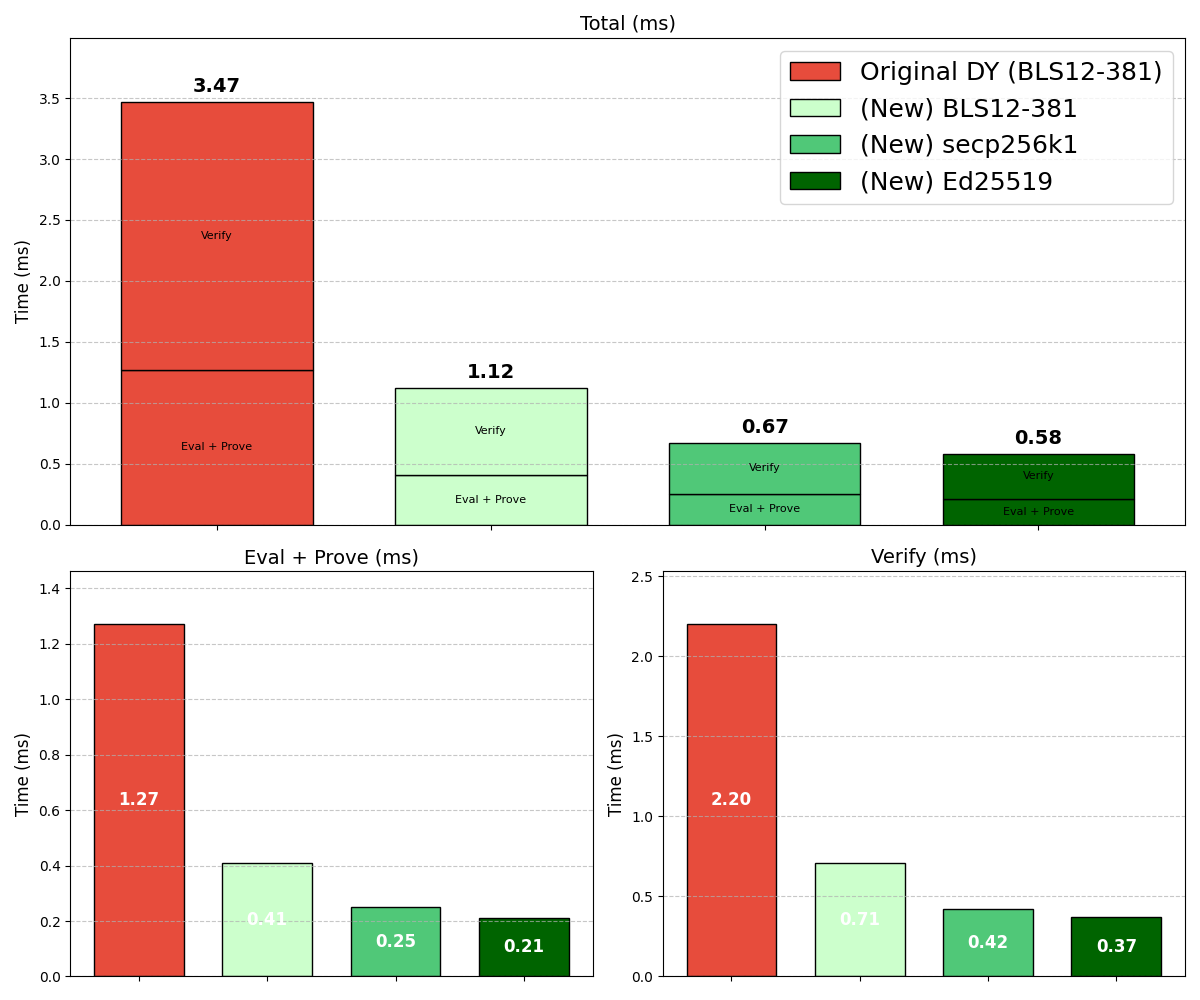
\includegraphics[width=1\linewidth]{figures/chap4_dy_comparisons.png}
        \caption[Our DY VRF Construction is 3 - 6x more efficient]{DY VRF Performance Comparison - Our Construction is 3 - 6x more efficient}
    \label{fig:chap4_public_vrf}
\end{figure}

% \begin{table}[!ht]\label{chap4_table_originaldy_vs_mydy}
% \begin{center}
% \caption{VRF Comparison between Original DY and Our Prime Order DY VRF Construction}
% \label{tab:chap4_vrf_public_table}
% \begin{tabular}{l@{\hspace{1em}}l@{\hspace{1em}}c@{\hspace{2em}}c@{\hspace{1em}}c}
% \toprule
% \textbf{Scheme} & \textbf{Curve} & \textbf{Eval + Prove (ms)} & \textbf{Verify (ms)} & \textbf{Total (ms)}\\
% \midrule
% \multirow{3}{*}{My DY Construction\ref{sec-dy-pf}} 
% & Ed25519 & 0.21 & 0.37 & 0.58\\
% & secp256k1 & 0.25 & 0.42 & 0.67\\
% & BLS12-381 & 0.41 & 0.71 & 1.12 \\
% \midrule
% Original DY $^1$ \cite{hutchison_verifiable_2005} & BLS12-381 & 1.27 & 2.27 & 3.54 \\
% \bottomrule
% \end{tabular}
% \par\medskip
% \raggedright
% \footnotesize{$^1$We use optimized pairing for verification by computing all pairings in Miller Loop format before a single Final Exponentiation, reducing verify time from 2.85(ms) to 2.27(ms), a 1.26x speedup.}
% \end{center}
% \end{table}

































\clearpage
\section{Private Nullifiers from the q-DDHI}\label{sec:privacy-preserving-vrf}

While our pairing-free VRF construction, presented in Section 3, eliminates the computational overhead of bilinear pairings, it still exposes the public key $pk = g^{sk}$ and input $x$ during verification. This is a limitation for anonymous credential systems, where both the master credential key $sk$ and the context identifier $x$ must remain private to ensure user anonymity. In this section, we address this challenge by developing zero-knowledge proof techniques that enable verification of VRF outputs computed from committed attributes, without revealing sensitive information.



Our approach builds progressively across three key stages:

\begin{enumerate}
    \item \textbf{Proving Knowledge of a Committed Inverse Exponent}: We start with a foundational protocol to prove that a value $y = g^{1/x}$ corresponds to a committed exponent $x$, leveraging the $q$-DDHI assumption. This establishes the base for our next protocols.

    \item \textbf{Proving Knowledge of a Committed Inverse Linear Relation}: We extend this technique to handle linear combinations of committed values, enabling verification of a VRF output $y = g^{1/(sk + x)}$ where $sk$ and $x$ are committed in separate credentials. This deterministic nullifier supports privacy-preserving credential binding and sybil resistance.

    \item \textbf{Proving Knowledge of a Committed Nullifier}: Finally, we introduce a protocol to commit to the VRF output itself (i.e., $\cm_y = g_3^{1/(sk + x)} g^{r_3}$), allowing unlinkable presentations. This probabilistic nullifier ensures that repeated uses of the same credential relationship remain unlinkable while still verifiable.
\end{enumerate}

These protocols collectively transform our prime-order VRF into a privacy-preserving tool suitable for hierarchical anonymous credential systems. In the subsections that follow, we detail each stage, presenting the cryptographic constructions and their security properties. \ref{chap5} will later demonstrate how these building blocks are instantiated for sybil resistance and revocation in the Multi-Issuer Multi-Credential (MIMC) system.







\subsection{Technical Challenge: Proving Knowledge of the q-DHHI challenge}

The central challenge in constructing a pairing-free VRF lies in verifying the correctness of an inverse relationship, specifically that $y = g^{1/x}$ for committed values, without relying on bilinear pairings. In standard prime-order group cryptography, while computing $g^x$ is straightforward, directly verifying $g^{1/x}$ is not, as pairings typically enable this through $e(g^x, g^{1/x}) = e(g,g)$. Our key insight is to reformulate this verification by proving an equivalent relationship: $y^x = g$. This equivalence holds because if $y = g^{1/x}$, then $y^x = (g^{1/x})^x = g^{(1/x) \cdot x} = g$, and conversely, if $y^x = g$, then $y = g^{1/x}$ (assuming $x \neq 0 \mod q$). This transformation eliminates the need for pairings by enabling verification via standard exponentiation, which can be efficiently proven using zero-knowledge techniques.

The protocol we present leverages this equivalence through a zero-knowledge proof where the prover demonstrates knowledge of the opening of a commitment $\cm = g_1^x g^r$ while simultaneously proving that $y^x = g$. This dual verification ensures that $y$ correctly encodes the inverse of $x$ without revealing $x$, forming a foundation for our pairing-free VRF that balances efficiency and privacy.

\subsection{Our Sigma-Protocol: Proving Knowledge of a Committed Inverse Exponent}

We begin with a simplified relation: given a commitment $\cm = g_1^x g^r$ and an element $y = g^{1/x}$, the prover demonstrates knowledge of $x$ and $r$ satisfying both equations, without revealing them. This is linked to the Decisional Diffie-Hellman Inversion (DDHI) assumption—where distinguishing $g^{1/x}$ from a random element given $g, g^x$ is computationally hard—making it a secure and essential starting point for our privacy-preserving construction.


\begin{protocol}{Proving Knowledge of Inverse Exponent}{committed-inverse-exponent}\label{pok-committed-inverse-exponent}
\textbf{Common Input:} Group generators $g_1, g \in \mathbb{G}$, commitment $\cm \in \mathbb{G}$, and element $y \in \mathbb{G}$ \\
\textbf{Prover Input:} Witness $(x, r)$ such that $\cm = g_1^x g^r$ and $y = g^{1/x}$ \\
\textbf{Relation:} 
\[
\mathcal{R}_{\mathsf{DDHI}} = \left\{ (\cm, y), (x, r) \ \middle|\ \cm = g_1^x g^r \ \land\ y = g^{1/x} \right\}
\]
\begin{enumerate}
    \item \textbf{Commitment:} Prover samples $a_x, a_r \sample \mathbb{Z}_q$ and computes:
    \[
    T_1 = g_1^{a_x} g^{a_r}, \quad T_y = y^{a_x}
    \]
    Sends $(T_1, T_y)$ to the verifier.

    \item \textbf{Challenge:} Verifier samples $c  \sample  \mathbb{Z}_q$ and sends $c$ to the prover.

    \item \textbf{Response:} Prover computes:
    \[
    z_x = a_x + c \cdot x, \quad z_r = a_r + c \cdot r
    \]
    Sends $(z_x, z_r)$ to the verifier.

    \item \textbf{Verification:} Verifier checks:
    \[
    T_1 \cdot \cm^c \stackrel{?}{=} g_1^{z_x} g^{z_r}, \quad T_y \cdot g^c \stackrel{?}{=} y^{z_x}
    \]
\end{enumerate}
\end{protocol}



This protocol achieves two objectives simultaneously:
\begin{enumerate}
    \item The first verification equation ($T_1 \cdot \cm^c \stackrel{?}{=} g_1^{z_x} g^{z_r}$) proves the prover knows a valid opening $(x, r)$ of the commitment $\cm$. This is a standard Schnorr-type proof for Pedersen commitments.
    
    \item The second equation ($T_y \cdot g^c \stackrel{?}{=} y^{z_x}$) verifies that $y^x = g$, which means $y = g^{1/x}$. This is the critical link proving that $y$ is correctly computed as the inverse exponent.
\end{enumerate}


\subsubsection{Security Analysis}


\begin{theorem}
Protocol~\ref{pok-committed-inverse-exponent} is a $\Sigma$-protocol for $\mathcal{R}_{\mathsf{DDHI}}$.
\end{theorem}

\begin{proof}[Sketch]
We verify the three properties of a $\Sigma$-protocol:

\begin{itemize}
    \item \textbf{Completeness:} For an honest prover with witness $(x, r)$, the verification equations hold:
          $$T_1 \cdot \cm^c = g_1^{z_x} g^{z_r} \quad \text{and} \quad T_y \cdot g^c = y^{z_x},$$
          as they are satisfied by the protocol's construction.
    
    \item \textbf{Special Soundness:} Given two accepting transcripts $(T_1, T_y, c, z_x, z_r)$ and $(T_1, T_y, c', z_x', z_r')$ with $c \neq c'$, we can extract:
          $$x = \frac{z_x - z_x'}{c - c'} \quad \text{and} \quad r = \frac{z_r - z_r'}{c - c'},$$
          such that $\cm = g_1^x g^r$ and $y^x = g$.
    
    \item \textbf{Honest-Verifier Zero-Knowledge (HVZK):} A simulator samples $z_x, z_r \in \mathbb{Z}_q$ and computes:
          $$T_1 = g_1^{z_x} g^{z_r} \cdot \cm^{-c} \quad \text{and} \quad T_y = y^{z_x} \cdot g^{-c},$$
          yielding a transcript indistinguishable from a real one.
\end{itemize}
\end{proof}

\paragraph{Relation to $q$-DDHI Assumption.}  The $q$-DDHI assumption ensures that $g^{1/x}$ is computationally indistinguishable from random elements when $x$ is hidden. However, pseudorandomness requires outputs remain indistinguishable even after seeing multiple input-output pairs from the same secret key, and therefore $y = g^{1/x}$ is not pseudorandom.


















\subsection{Our Sigma-Protocol: Proving Knowledge of a Committed Inverse Linear Relation}\label{sec-pok-committed-inv-linear-relation}

We now address proving inverse relationships involving linear combinations of committed values. Specifically, we prove knowledge of $(sk, x, r_1, r_2)$ such that:

\[
\mathcal{R}_{\mathsf{nullifier}} = \left\{ 
\begin{array}{l} (\cm_1, \cm_2, y),\\
(sk, x, r_1, r_2) 
\end{array}
\ \middle|
\ \begin{array}{l}
\cm_1 = g_1^{sk} g^{r_1} \\
\cm_2 = g_2^{x} g^{r_2} \\
y = g^{1/(sk + x)} \\
\end{array} \right\}
\]







\subsubsection{Construction}
The protocol extends our single-commitment construction by (1) proving knowledge of openings for $\cm_1$ and $\cm_2$ simultaneously, and (2) verifying $y^{sk+x} = g$ where $sk+x$ combines values from distinct commitments. The consistency check $z_m = z_{sk} + z_x$ prevents substitution attacks where an adversary might use different linear combinations across verification equations.

\begin{protocol}{Proving Committed Inverse Linear Relation}{}\label{pok-committed-inverse-linear-relation}
\textbf{Common Input:} Group generators $g_1, g_2, g \in \mathbb{G}$, $\cm_1, \cm_2, y \in \mathbb{G}$ \\
\textbf{Prover Input:} Witness $(sk, x, \usk_1, \usk_2)$ such that $\cm_1 = g_1^{sk} g^{\usk_1}$, $\cm_2 = g_2^{x}g^{\usk_2}$ and $ y = g^{1/(sk + x)}$ \\
\textbf{Relation: }
\[
\mathcal{R} = \{(\cm_1,\cm_2, y), (sk, x, \usk_1, \usk_2) \mid \cm_1 = g_1^{sk} g^{\usk} \wedge \cm_2 = g_2^{x}g^{\usk_2} \wedge y = g^{1/(sk + x)}\}
\]
\begin{enumerate}
    \item \textbf{Commitment:} Prover computes:
    \begin{align*}
        a_{sk}, a_x, a_{r_1}, a_{r_2} &\sample \Z_q & T_1 &\gets g_1^{a_{sk}} g^{a_{r_1}} & T_2 &\gets g_2^{a_x} g^{a_{r_2}} & T_y &\gets y^{a_{sk} + a_x}
    \end{align*}
    Sends $(T_1, T_2, T_y)$ to verifier.
    
    \item \textbf{Challenge:} Verifier samples $c \sample \mathbb{Z}_q$ and sends to prover.
    
    \item \textbf{Response:} Prover computes:
     \begin{align*}
        z_{sk} &= a_{sk} + c \cdot sk & z_x &= a_x + c \cdot x &  z_m &= (a_{sk} + a_x) + c \cdot (sk + x)\\   
        z_{r_1} &= a_{r_1} + c \cdot r_1 & z_{r_2} &= a_{r_2} + c \cdot r_2
    \end{align*}
    Sends $(z_{sk}, z_x, z_{r_1} z_{r_2}, z_m)$ to verifier.
    
    \item \textbf{Verification:} Verifier checks:
    \begin{align*}
        T_1 \cdot \cm_1^c &\stackrel{?}{=} g_1^{z_{sk}}g^{z_{r_1}} 
        &
        T_2 \cdot \cm_2^c &\stackrel{?}{=}  g_2^{z_x} g^{z_{r_2}} 
        &
        T_y \cdot g^c &\stackrel{?}{=} y^{z_m} &
        z_m &\stackrel{?}{=} z_{sk} + z_x
    \end{align*}
\end{enumerate}
\end{protocol}


\subsubsection{Security Analysis}

\begin{theorem}
Protocol~\ref{pok-committed-inverse-linear-relation} is a $\Sigma$-protocol for $\mathcal{R}_{\mathsf{nullifier}}$.
\end{theorem}

\begin{proof}[Sketch]
\begin{itemize}
    \item \textbf{Completeness:} For an honest prover, all verification equations hold by similar derivations to the basic case, with the additional consistency check $z_m = z_{sk} + z_x$ holding by construction.
    
    \item \textbf{Special Soundness:} From accepting transcripts $(T_1, T_2, T_y, c, z_{sk}, z_x, z_{r_1}, z_{r_2}, z_m)$ and \\ $(T_1, T_2, T_y, c', z'_{sk}, z'_x, z'_{r_1}, z'_{r_2}, z'_m)$ with $c \neq c'$, extract $sk = \frac{z_{sk} - z'_{sk}}{c - c'}$, etc. The third verification equation yields $y^{(c - c')(sk + x)} = g^{c - c'}$, thus $y^{sk+x} = g$.

    \item \textbf{HVZK:} Simulator samples $z_{sk}, z_x, z_{r_1}, z_{r_2} \sample \mathbb{Z}_q$, sets $z_m = z_{sk} + z_x$, computes $T_1 = g_1^{z_{sk}}g^{z_{r_1}} \cdot \cm_1^{-c}$, etc.
\end{itemize}
\end{proof}








\subsection{We Construct a Deterministic Nullifier from \ref{sec-pok-committed-inv-linear-relation}}
\label{subsec:deterministic-nullifier}

Our VRF operates in a prime-order group $\mathbb{G}$ of order $p$ with generators $g_1, g_2, g_3, g$. The message space is $ x \in \mathcal{X} = \Z_p^*$, the output space is $y \in \mathcal{Y} = \Z_p^*$, and the proof space is $\pi \in \Pi\ = \mathbb{G} \times \mathbb{G} \times \mathbb{Z}_p$. We assume the existence of $\cm_1 = g_1^{sk} g^{r_1}$ and $\cm_2 = g_2^{x} g^{r_2}$.

The algorithms are defined as follows

\begin{itemize}
    \item $\mathsf{dVRF.Eval}(sk, x) \to y$: $y = g_3^{1/(sk+x)}$
    
    \item $\mathsf{dVRF.Prove}(\cm_1, \cm_2, sk, x, y) \to \pi$: Run protocol ~\ref{pok-committed-inverse-linear-relation}, output $\pi, \cm_y$
    
    \item $\mathsf{dVRF.Verify}(\cm_1, \cm_2, y, \pi) \to \{0,1\}$: Output 1 if $\pi$ verifies $\cm_1, \cm_2, y$ correctly per the $\Sigma$-protocol \ref{pok-committed-inverse-linear-relation}, else 0.
\end{itemize}



\subsubsection{Security Properties}

\begin{theorem}[Correctness]
The deterministic nullifier VRF is correct: for all $\lambda \in \mathbb{N}$, $\mathsf{pp} \in \mathsf{Setup}(1^\lambda)$, $(\mathsf{sk}, \mathsf{pk}) \in \mathsf{VRF.Gen}(\mathsf{pp})$, $x \in \mathbb{Z}_p$, and $\cm_2 = g_2^{x} g^{r_2}$:
\[
\Pr[\mathsf{dVRF.Verify}(\cm_1, \cm_2, \mathsf{dVRF.Eval}(\mathsf{sk}, x), \mathsf{dVRF.Prove}(\cm_1, \cm_2, sk, x, y)) = 1] = 1
\]
\end{theorem}

\begin{proof}
Correctness follows directly from the completeness of Protocol~\ref{pok-committed-inverse-linear-relation}. Since honest execution ensures all verification equations in the underlying Sigma protocol hold, the VRF verification checks pass.
\end{proof}

\begin{theorem}[Uniqueness]
Under the binding property of Pedersen commitments and the discrete logarithm assumption, for any $\cm_1$ and $\cm_2$, there exists at most one $y \in \mathbb{G}$ such that $\mathsf{dVRF.Verify}(\cm_1, \cm_2, y, \pi) = 1$ for any $\pi$.
\end{theorem}

\begin{proof}[Sketch]
The binding property of Pedersen commitments ensures that $\cm_1$ commits to $sk$ and $\cm_2$ commits to $x$ uniquely. Therefore, $y = g^{1/(sk + x)}$ is uniquely determined. If two different values $y' \neq y$ could verify, special soundness would extract witnesses satisfying both $y^{sk+x} = g$ and $y'^{sk+x} = g$, implying $(y'/y)^{sk+x} = 1$. In a prime-order group, this holds only if $y' = y$ or $sk + x \equiv 0 \pmod{p}$. The latter occurs with negligible probability for randomly chosen $sk$ and $x$.
\end{proof}

\begin{theorem}[Pseudorandomness]
Under the $q$-DDHI assumption, the deterministic nullifier VRF satisfies pseudorandomness. For any PPT adversary $\mathcal{A}$:
\[
\mathsf{Adv}^{\mathsf{vrf}}_{\mathcal{A}}(\lambda) \leq \mathsf{Adv}^{\mathsf{q-DDHI}}(\lambda) + \mathsf{negl}(\lambda)
\]
\end{theorem}

\begin{proof}[Sketch]
We construct a reduction $\mathcal{B}$ that uses $\mathcal{A}$ to solve $q$-DDHI:
\begin{enumerate}
    \item $\mathcal{B}$ receives a $q$-DDHI challenge $(g, g^a, \ldots, g^{a^q}, Z)$ where $Z$ is either $g^{1/a}$ or random
    \item $\mathcal{B}$ embeds $a$ as $sk$ by setting $\mathsf{pk} = \cm_1 = g_1^a \cdot g^{r_1}$
    \item For evaluation queries on $x_i$, $\mathcal{B}$ computes $y_i = g^{1/(a+x_i)}$ using the $q$-DDHI instance
    \item For the challenge $x^*$, $\mathcal{B}$ returns $y^* = Z^{1/(a+x^*)}$
    \item By the HVZK property of the Sigma protocol, $\mathcal{B}$ simulates proofs
    \item If $\mathcal{A}$ distinguishes, $\mathcal{B}$ solves the $q$-DDHI challenge
\end{enumerate}
The advantage is bounded by the $q$-DDHI advantage plus the negligible HVZK simulation error.
\end{proof}























\subsection{Our Sigma-Protocol: Proving Knowledge of a Committed Inverse Linear Relation}\label{chap4:pok_committed_inverse_linear_relation}

A deterministic nullifier $y = g^{1/(sk + x)}$ is essential for sybil resistance, ensuring a unique, verifiable value for each $(sk, x)$ pair derived from a master credential key $sk$ and context identifier $x$. However, revealing the nullifier directly introduces linkability risks, as each presentation exposes a deterministic function of $(sk, x)$, potentially allowing user actions to be tracked across interactions. To resolve this, we construct a zero-knowledge Sigma-protocol that proves knowledge of a nullifier embedded within a Pedersen commitment, enabling unlinkable presentations while preserving the verifiable binding necessary for security.

Our solution commits to the nullifier as:
\[
\cm_{\text{null}} = g_3^{1/(sk + x)} g^{r_3}
\]
where $r_3 \sample \mathbb{Z}_q$ provides fresh randomness for each presentation, ensuring unlinkability. We then design a protocol to prove that $\cm_{\text{null}}$ correctly commits to $g_3^{1/(sk + x)}$, where $sk$ and $x$ are themselves committed in $\cm_1 = g_1^{sk} g^{r_1}$ and $\cm_2 = g_2^{x} g^{r_2}$, without revealing any of these values. This approach supports privacy-preserving applications like revocation and set membership proofs in the Multi-Issuer Multi-Credential (MIMC) system.

The key innovation is an auxiliary commitment $\cm_4 = \cm_3^{sk + x} g^{r_4} = g_3 g^{r_3 (sk + x) + r_4}$, which allows us to verify that $\cm_3^{sk + x} = g_3$ (modulo randomness) in zero knowledge. This algebraic structure ensures the nullifier’s correctness while operating entirely within the commitment space.

\begin{protocol}{Proof of Committed Nullifier}{}
\label{prot:committed-nullifier}
\textbf{Public parameters:} Prime-order group $\mathbb{G}$ with generators $g_1, g_2, g_3, g \in \mathbb{G}$\\
\textbf{Common input:} $(\cm_1, \cm_2, \cm_3, \cm_4) \in \mathbb{G}^4$\\
\textbf{Prover input:} $(sk, x, r_1, r_2, r_3, r_4) \in \mathbb{Z}_p^6$  \\
\textbf{Relation:} 
\[
\mathcal{R}_{\mathsf{CN}} = \left\{ 
\begin{array}{l} 
(\cm_1, \cm_2, \cm_3, \cm_4), \\
(sk, x, r_1, r_2, r_3, r_4) 
\end{array}
\ \middle| \
\begin{array}{l}
\cm_1 = g_1^{sk} g^{r_1} \\
\cm_2 = g_2^{x} g^{r_2} \\
\cm_3 = g_3^{1/(sk + x)} g^{r_3}  \quad \text{\small{(committed nullifier)}}\\
\cm_4 = g_3 g^{r_3 (sk + x) + r_4}  \quad \text{\small{(auxiliary commitment)}}
\end{array} \right\}
\]
\begin{enumerate}
    \item \textbf{Prover} samples $a_{sk}, a_x, a_{r_1}, a_{r_2}, a_{r_3}, a_{r_4} \sample \mathbb{Z}_p$ and computes:
    \begin{align*}
        T_1 &= g_1^{a_{sk}} g^{a_{r_1}} & T_2 &= g_2^{a_x} g^{a_{r_2}} &
        T_3 &= g_3^{a_{\beta}} g^{a_{r_3}} & T_4 &= \cm_3^{a_m} g^{a_{r_4}}
    \end{align*}
    where $a_m = a_{sk} + a_x$ and $a_{\beta} = \frac{1}{a_m}$. Sends $(T_1, T_2, T_3, T_4)$.
    
    \item \textbf{Verifier} sends challenge $c \sample \mathbb{Z}_p$.
    
    \item \textbf{Prover} computes and sends:
    \begin{align*}
        z_{sk} &= a_{sk} + c \cdot sk & z_x &= a_x + c \cdot x &  z_{r_i} &= a_{r_i} + c \cdot r_i \text{ for } i \in \{1,2,3,4\} \\
        z_m &= a_m + c \cdot (sk + x) & z_{\beta} &= a_{\beta} + c \cdot \frac{1}{sk + x}
    \end{align*}
    
    \item \textbf{Verifier} accepts iff:
    \begin{align*}
        T_1 \cdot \cm_1^c &= g_1^{z_{sk}} g^{z_{r_1}} 
        & 
        T_2 \cdot \cm_2^c &= g_2^{z_x} g^{z_{r_2}} 
        &
        T_3 \cdot \cm_3^c &= g_3^{z_{\beta}} g^{z_{r_3}} \\
        T_4 \cdot \cm_4^c &= \cm_3^{z_m} g^{z_{r_4}}
        &
        z_m &= z_{sk} + z_x
    \end{align*}
\end{enumerate}
\end{protocol}



\subsubsection{Security Analysis}
We establish the security of our protocol by proving three core properties: completeness, special soundness, and honest-verifier zero-knowledge (HVZK). These properties ensure that the protocol is correct, extractable, and privacy-preserving, respectively.

\paragraph{Completeness}
Completeness guarantees that an honest prover, using the correct witness $(sk, x, r_1, r_2, r_3, r_4)$ satisfying the relation $\mathcal{R}_{\mathsf{CN}}$, always convinces the verifier. We verify each step of the protocol to confirm that all verification equations hold.

Assume the prover follows the protocol with:
\[
\cm_1 = g_1^{sk} g^{r_1}, \quad \cm_2 = g_2^{x} g^{r_2}, \quad \cm_3 = g_3^{1/(sk + x)} g^{r_3}, \quad \cm_4 = g_3 g^{r_3 (sk + x) + r_4}
\]
and samples $a_{sk}, a_x, a_{r_1}, a_{r_2}, a_{r_3}, a_{r_4} \sample \mathbb{Z}_p$. Let $a_m = a_{sk} + a_x$ and $a_{\beta} = \frac{1}{a_m}$, assuming $a_m \neq 0 \pmod{p}$


The prover computes:
\[
T_1 = g_1^{a_{sk}} g^{a_{r_1}}, \quad T_2 = g_2^{a_x} g^{a_{r_2}}, \quad T_3 = g_3^{a_{\beta}} g^{a_{r_3}}, \quad T_4 = \cm_3^{a_m} g^{a_{r_4}}
\]
After receiving challenge $c$, the prover sends:
\[
z_{sk} = a_{sk} + c \cdot sk, \quad z_x = a_x + c \cdot x, \quad z_{r_i} = a_{r_i} + c \cdot r_i \text{ for } i \in \{1,2,3,4\}, \quad z_m = a_m + c \cdot (sk + x), \quad z_{\beta} = a_{\beta} + c \cdot \frac{1}{sk + x}
\]

The verifier checks:
\begin{enumerate}
    \item $T_1 \cdot \cm_1^c \stackrel{?}{=} g_1^{z_{sk}} g^{z_{r_1}}$
    \[
    1) \qquad T_1 \cdot \cm_1^c = g_1^{a_{sk}} g^{a_{r_1}} \cdot (g_1^{sk} g^{r_1})^c = g_1^{a_{sk} + c \cdot sk} g^{a_{r_1} + c \cdot r_1} = g_1^{z_{sk}} g^{z_{r_1}}
    \]
    \item $T_2 \cdot \cm_2^c \stackrel{?}{=} g_2^{z_x} g^{z_{r_2}}$
    \[
    T_2 \cdot \cm_2^c = g_2^{a_x} g^{a_{r_2}} \cdot (g_2^{x} g^{r_2})^c = g_2^{a_x + c \cdot x} g^{a_{r_2} + c \cdot r_2} = g_2^{z_x} g^{z_{r_2}}
    \]
    \item $T_3 \cdot \cm_3^c \stackrel{?}{=} g_3^{z_{\beta}} g^{z_{r_3}}$
    \[
    T_3 \cdot \cm_3^c = g_3^{a_{\beta}} g^{a_{r_3}} \cdot (g_3^{1/(sk + x)} g^{r_3})^c = g_3^{a_{\beta} + c / (sk + x)} g^{a_{r_3} + c \cdot r_3} = g_3^{z_{\beta}} g^{z_{r_3}}
    \]
    \item $T_4 \cdot \cm_4^c \stackrel{?}{=} \cm_3^{z_m} g^{z_{r_4}}$
    \[
    T_4 \cdot \cm_4^c = \cm_3^{a_m} g^{a_{r_4}} \cdot (g_3 g^{r_3 (sk + x) + r_4})^c = \cm_3^{a_m} g^{a_{r_4}} \cdot g_3^c g^{c (r_3 (sk + x) + r_4)}
    \]
    Since $\cm_3^{sk + x} = g_3 g^{r_3 (sk + x)}$ and $\cm_4 = \cm_3^{sk + x} g^{r_4}$, we have:
    \[
    T_4 \cdot \cm_4^c = \cm_3^{a_m} g^{a_{r_4}} \cdot (\cm_3^{sk + x} g^{r_4})^c = \cm_3^{a_m + c (sk + x)} g^{a_{r_4} + c r_4} = \cm_3^{z_m} g^{z_{r_4}}
    \]
    \item $z_m \stackrel{?}{=} z_{sk} + z_x$
    \[
    z_m = a_m + c (sk + x) = (a_{sk} + a_x) + c (sk + x) = z_{sk} + z_x
    \]
\end{enumerate}
All equations hold, confirming completeness.

\paragraph{Special Soundness}
Given two accepting transcripts with distinct challenges $c \neq c'$, we extract:
\[
sk = \frac{z_{sk} - z_{sk}'}{c - c'}, \quad x = \frac{z_x - z_x'}{c - c'}, \quad r_i = \frac{z_{r_i} - z_{r_i}'}{c - c'} \text{ for } i \in \{1,2,3,4\}
\]
From $z_{\beta} = a_{\beta} + c \cdot \frac{1}{sk + x}$ and $z_{\beta}' = a_{\beta} + c' \cdot \frac{1}{sk + x}$, we derive $\frac{1}{sk + x} = \frac{z_{\beta} - z_{\beta}'}{c - c'}$, ensuring $\cm_3$ commits to $g_3^{1/(sk + x)} g^{r_3}$. This confirms extractability.

\paragraph{Honest-Verifier Zero-Knowledge (HVZK)}
A simulator samples $z_{sk}, z_x, z_{r_1}, z_{r_2}, z_{r_3}, z_{r_4}, z_m, z_{\beta} \sample \mathbb{Z}_p$ and computes:
\[
T_1 = g_1^{z_{sk}} g^{z_{r_1}} \cdot \cm_1^{-c}, \quad T_2 = g_2^{z_x} g^{z_{r_2}} \cdot \cm_2^{-c}, \quad T_3 = g_3^{z_{\beta}} g^{z_{r_3}} \cdot \cm_3^{-c}, \quad T_4 = \cm_3^{z_m} g^{z_{r_4}} \cdot \cm_4^{-c}
\]
These satisfy the verification equations, and the simulated transcript’s distribution matches the real one, ensuring zero-knowledge.






































\subsection{We Construct a Probabilistic Nullifier from \ref{chap4:pok_committed_inverse_linear_relation}}\label{sec-probabilistic-nullifier}

\subsubsection{Algorithm Syntax}
Here, the output is a commitment $\cm_y = g_3^{1/(sk + x)} g^{r_3}$, randomized per presentation, with an auxiliary commitment $\cm_4$ for verification.

\begin{itemize}
    \item $\mathsf{pVRF.Eval}(sk, x) \to \cm_y$: Sample $r_3 \sample \Z_p^*$, compute $\cm_y = g_3^{1/(sk+x)}g^{r_3}$, sample $r_4 \sample \Z_p^*$ compute $\cm_4 = g_3g^{r_3 \cdot (sk+x) + r_4}$ return $\cm_y, \cm_4$
    
    \item $\mathsf{pVRF.Prove}(\cm_1, \cm_2, \cm_y, \cm_4, sk, x, r_1, \ldots, r_4) \to \pi$: Run protocol ~\ref{pok-committed-inverse-linear-relation}, output $\pi$
    
    \item $\mathsf{pVRF.Verify}(\cm_1, \cm_2, \cm_y, \cm_4, \pi) \to \{0,1\}$: Output 1 if $\pi$ verifies $\cm_1, \cm_2, \cm_y, \cm_4$ correctly per the $\Sigma$-protocol \ref{prot:committed-nullifier}, else 0.
\end{itemize}




\subsubsection{Security Properties}

\begin{theorem}[Correctness]
The probabilistic nullifier VRF is correct following from the completeness of Protocol~\ref{prot:committed-nullifier}.
\end{theorem}

\begin{theorem}[Uniqueness]
For fixed $\mathsf{pk}$ and $\cm_2$, the underlying nullifier value $g^{1/(sk + x)}$ is unique, though committed differently each time. The binding property of commitments ensures $sk$ and $x$ are uniquely determined.
\end{theorem}

\begin{theorem}[Unlinkability]
For any PPT adversary $\mathcal{A}$ making polynomially many queries, the following experiment has negligible advantage:
\[
\mathsf{Adv}^{\mathsf{unlink}}_{\mathcal{A}}(\lambda) = \left| \Pr[\mathsf{Exp}^{\mathsf{unlink-1}}_{\mathcal{A}}(\lambda) = 1] - \Pr[\mathsf{Exp}^{\mathsf{unlink-0}}_{\mathcal{A}}(\lambda) = 1] \right| \leq \mathsf{negl}(\lambda)
\]
where $\mathsf{Exp}^{\mathsf{unlink-b}}$ is:
\begin{enumerate}
    \item $\mathcal{A}$ chooses $(\mathsf{pk}, \cm_{2,0}, \cm_{2,1})$ where $\cm_{2,0}, \cm_{2,1}$ commit to the same $x$
    \item Challenger computes $(\cm_{y,b}, \pi_b) \leftarrow \mathsf{VRF.Eval}(\mathsf{sk}, x), \mathsf{VRF.Prove}(\mathsf{sk}, x, \cm_{2,b})$
    \item $\mathcal{A}$ outputs $b'$ given $(\cm_{y,b}, \pi_b)$
\end{enumerate}
\end{theorem}

\begin{proof}[Sketch]
Unlinkability follows from:
\begin{enumerate}
    \item The hiding property of Pedersen commitments with fresh randomness $r_3, r_4$
    \item The HVZK property of Protocol~\ref{prot:committed-nullifier}, which reveals nothing beyond statement validity
    \item The statistical independence of commitments across presentations
\end{enumerate}
Each presentation uses independent randomness, making transcripts indistinguishable even for the same underlying $(sk, x)$ pair.
\end{proof}




















\section{Performance Evaluation}\label{sec:performance-vrf}

We implemented our constructions \cite{polgar_anonymous_2025} using the arkworks cryptography library \cite{arkworks_contributors_arkworks_2022} in Rust and evaluated performance on a MacBook Air M2 with 16GB RAM. Table~\ref{tab:performance-vrf} compares our constructions on BLS12-381 curve against baseline approaches, focusing on the critical operations of evaluation, proof generation, and verification. Table \ref{tab:performance-vrf-curves} shows our constructions built on different, non-pairing curves.

\begin{table}[ht]
\begin{center}
\caption{VRF Comparison with curve BLS12-381}
\label{tab:performance-vrf}
\begin{tabular}{l@{\hspace{1em}}c@{\hspace{1em}}r@{\hspace{2em}}r@{\hspace{5em}}r@{\hspace{2em}}r}
\toprule
\textbf{Scheme} & \textbf{Pairing} & \multicolumn{2}{c}{\textbf{Eval + Prove (ms)}} & \multicolumn{2}{c}{\textbf{Verify (ms)}} \\
\cmidrule(lr){3-4} \cmidrule(lr){5-6}
& & \textbf{ms} & \textbf{Speedup} & \textbf{ms} & \textbf{Speedup} \\
\midrule
DY $^1$ \cite{hutchison_verifiable_2005}                     & yes & 1.27 &  -      & 2.2   &  -     \\
Us (Prime Order DY) \ref{sec-dy-pf}                                   & no  & 0.41 & 3.1x   & 0.70  & 3.1x  \\
\midrule
DY Anonymous \cite{tomescu_utt_2022}                            & yes & 5.91 &   -     & 6.47  &   -    \\
Us (Anonymous + Deterministic) \ref{pok-committed-inverse-linear-relation} & no  & 1.08 & 5.5x   & 1.41  & 4.6x  \\
Us (Anonymous + Probabilistic) ~\ref{prot:committed-nullifier} & no  & 2.01 & 2.9x   & 1.65  & 3.9x  \\
\bottomrule
\end{tabular}
\par\medskip
\raggedright
\footnotesize{$^1$We use optimized pairing for verification by computing all pairings in Miller Loop format before a single Final Exponentiation, reducing verify time from 2.85(ms) to 2.27(ms), a 1.26x speedup.}
\end{center}
\end{table}

\begin{table}[ht]
\begin{center}
\caption{Performance of our VRF Constructions Across Elliptic Curves (time in ms)}
\label{tab:performance-vrf-curves}
\begin{tabular}{ll@{\hspace{1em}}r@{\hspace{1em}}r@{\hspace{3em}}r@{\hspace{1em}}r}
\toprule
\textbf{Curve} & \textbf{Scheme} & \multicolumn{2}{c}{\textbf{Eval + Prove}} & \multicolumn{2}{c}{\textbf{Verify}} \\
\cmidrule(lr){3-4} \cmidrule(lr){5-6}
& & \textbf{ms} & \textbf{Speedup} & \textbf{ms} & \textbf{Speedup} \\
\midrule
\multirow{3}{*}{BLS12-381} 
& Prime Order DY  \ref{sec-dy-pf} & 0.41 & - & 0.71 & - \\
& Prime Order, Anon. Deterministic \ref{pok-committed-inverse-linear-relation} & 1.15 & - & 1.08 & - \\
& Prime Order, Anon. Probabilistic ~\ref{prot:committed-nullifier} & 2.01 & - & 1.65 & - \\
\midrule
\multirow{3}{*}{Ed25519} 
&  Prime Order DY \ref{sec-dy-pf} & 0.21 & 2.0$\times$ & 0.37 & 1.9$\times$ \\
& Prime Order, Anon. Deterministic \ref{pok-committed-inverse-linear-relation} & 0.56 & 2.0$\times$ & 0.56 & 1.9$\times$ \\
& Prime Order, Anon. Probabilistic ~\ref{prot:committed-nullifier} & 1.04 & 1.9$\times$ & 0.84 & 2.0$\times$ \\
\midrule
\multirow{3}{*}{secp256k1} 
&  Prime Order DY \ref{sec-dy-pf} & 0.25 & 1.6$\times$ & 0.42 & 1.7$\times$ \\
& Prime Order, Anon. Deterministic \ref{pok-committed-inverse-linear-relation} & 0.66 & 1.8$\times$ & 0.66 & 1.6$\times$ \\
& Prime Order, Anon. Probabilistic ~\ref{prot:committed-nullifier} & 1.29 & 1.6$\times$ & 1.05 & 1.6$\times$ \\
\bottomrule
\end{tabular}
\par\medskip
\raggedright
\footnotesize{Measurements conducted on a MacBook Air M2 with 16GB RAM using the arkworks library \cite{arkworks_contributors_arkworks_2022} in Rust. Speedup is calculated relative to BLS12-381 for each scheme and operation. Times are rounded to two decimal places for clarity.}
\end{center}
\end{table}




Our evaluation reveals several key findings:

\begin{enumerate}
    \item \textbf{Pairing Elimination:} Our DY-PF construction achieves a 3.1× speedup over the original DY VRF by eliminating pairing operations, demonstrating the efficiency benefits of our approach.
    
    \item \textbf{Privacy Preservation Overhead:} Adding privacy preservation through commitments inevitably increases computational costs, but our DY-PF-Private design achieves a 5.5× speedup over comparable pairing-based private VRF schemes.
    
    \item \textbf{Unlinkability Trade-off:} The committed nullifier variant (DY-PF-Private-ComOut) involves additional operations for commitment handling, yet still maintains a 2.9× evaluation speedup and 3.9× verification speedup over pairing-based alternatives.

    \item \textbf{Inefficiency of Pairing Curve Operations} The non-pairing curve operations are from 1.6x - 2x more efficient
\end{enumerate}










% \begin{figure}[ht]
%     \centering
%     \begin{minipage}{\textwidth}
%         \centering
%         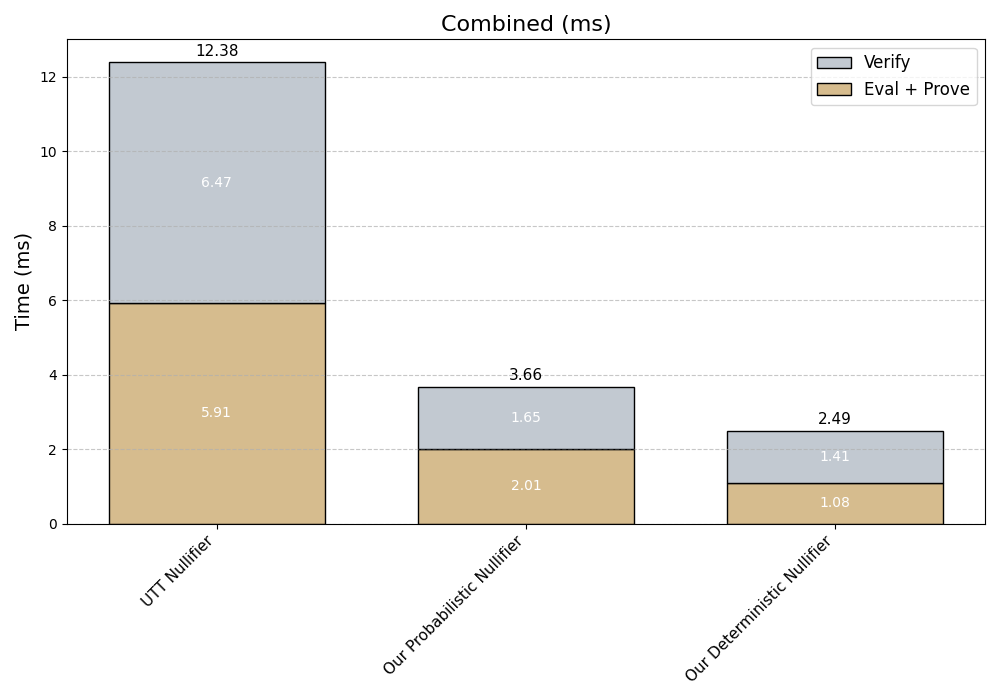
\includegraphics[width=0.75\textwidth]{figures/chap4_private_nullifier_combined.png}
%     \end{minipage}
    
%     % Bottom row with 2x2 grid of smaller figures
%     \begin{minipage}{0.48\textwidth}
%         \centering
%          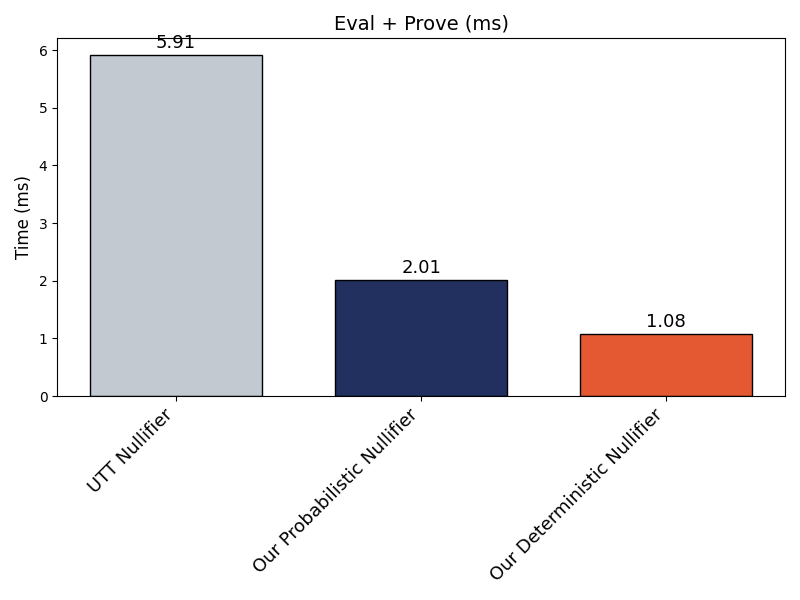
\includegraphics[width=\textwidth]{figures/chap4_private_nullifier_eval_prove.png}        
%     \end{minipage}
%     \hfill
%     \begin{minipage}{0.48\textwidth}
%         \centering
%        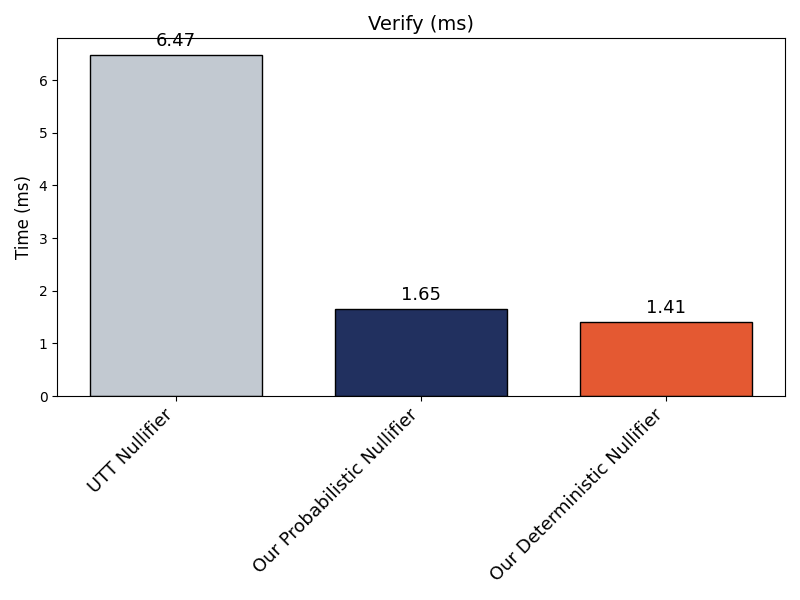
\includegraphics[width=\textwidth]{figures/chap4_private_nullifier_verify.png}
%     \end{minipage}
    
%     \caption[Our Nullifier Constructions are 3x - 5x more efficient]{Nullifier Performance Comparison - Our Constructions are 3x - 5x more efficient}
%     \label{fig:nullifiers_figure}
% \end{figure}




\begin{figure}[!htb]
    \centering
    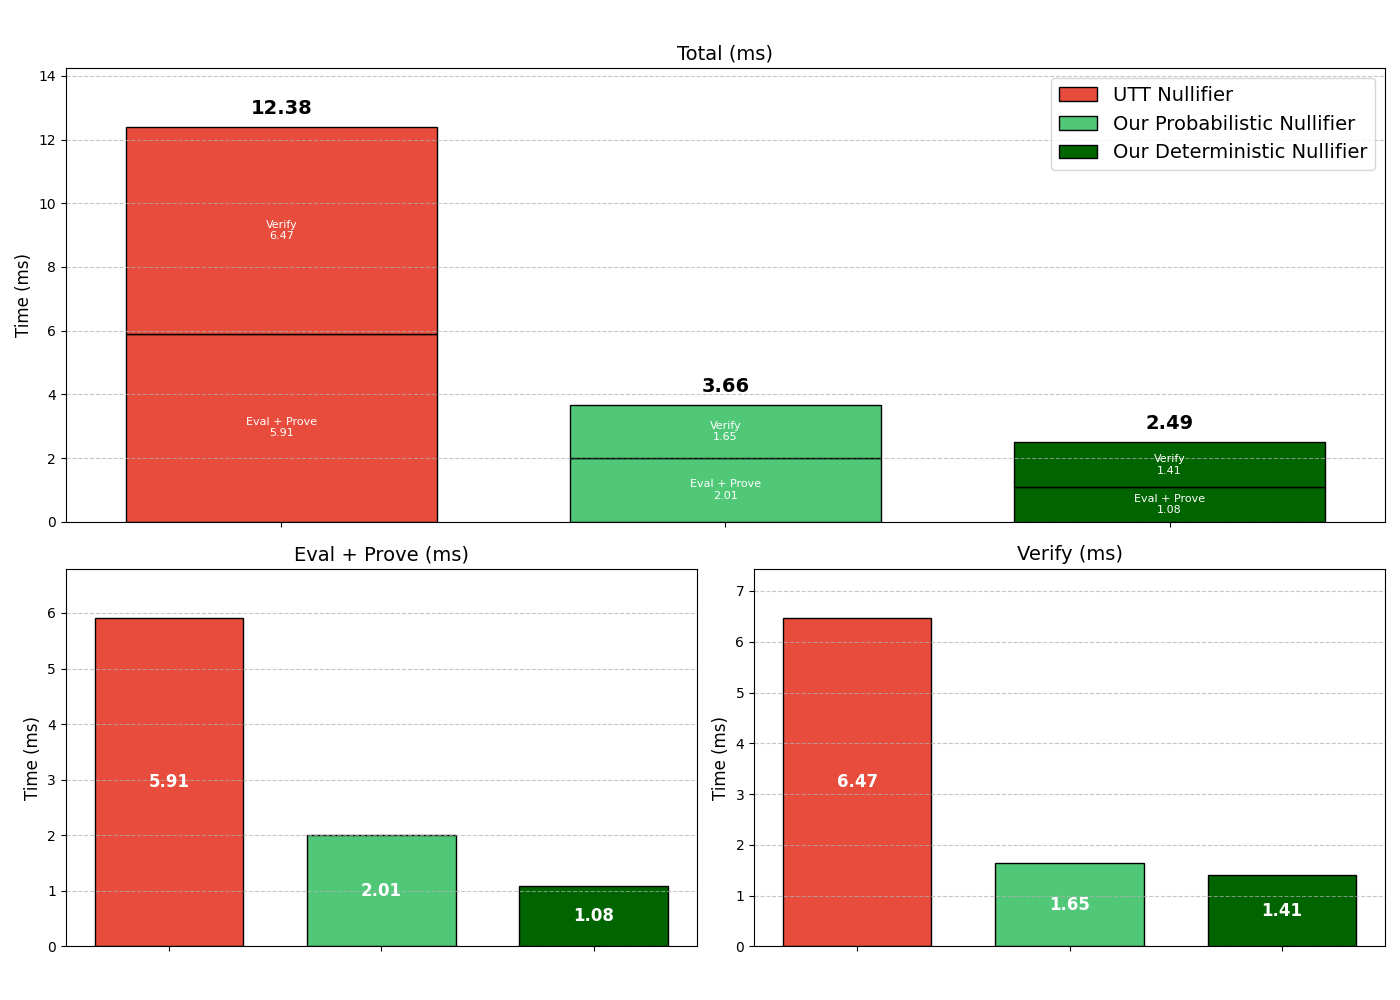
\includegraphics[width=1\linewidth]{figures/chap4_nullifier_comparisons.png}
    \caption[Our Nullifier Constructions are 3x - 5x more efficient]{Nullifier Performance Comparison - Our Constructions are 3x - 5x more efficient}
    \label{fig:nullifiers_figure}
\end{figure}

















\section{Instantiation: Anonymous Nullifiers for Sybil Resistance and Revocation}\label{sec-vrf-instantiation}

In this section, we instantiate the Credential Relationship Binding Nullifier (CRBN) within the Multi-Issuer Multi-Credential (MIMC) system, demonstrating its utility in real-world privacy-preserving identity frameworks. The CRBN leverages the prime-order, pairing-free Verifiable Random Function (VRF) constructions from Sections~\ref{sec:vrf-prime-order} and~\ref{sec:privacy-preserving-vrf} to provide efficient, anonymous nullifiers. We focus on two primary applications—sybil resistance and revocation—while highlighting additional use cases inspired by novel zkp applications. 

\subsection{Applications}\label{subsec:applications}

The CRBN enables a range of privacy-preserving applications by binding credentials hierarchically while enforcing uniqueness and revocability. Below, we outline key use cases:

\subsubsection{Sybil Resistance}\label{subsubsec:sybil-resistance}
Sybil resistance ensures that users cannot create multiple identities to exploit a system. The CRBN achieves this through its deterministic nullifier, $y = g^{1/(sk + x)}$, where $sk$ is the master credential key and $x$ is the context identifier (e.g., "DMV" for a driver's license). This nullifier is unique per user-context pair and verifiable via the zero-knowledge proof from Protocol~\ref{pok-committed-inverse-linear-relation}.

\textbf{Example: Anonymous Voting.} Consider a voting system where each user should vote once per election. A user with master credential key $sk$ computes $y = g^{1/(sk + x)}$ for election context $x$ (e.g., "Election2024"). They present $y$ with a zero-knowledge proof that it corresponds to a valid credential, without revealing $sk$ or $x$. The system maintains an anonymous user list (see Figure~\ref{fig:credential-nullifier-revised}) and rejects duplicate nullifiers, preventing double voting while preserving anonymity.

\subsubsection{Revocation}\label{subsubsec:revocation}
Revocation allows credentials to be invalidated without compromising privacy. Suppose an identity system has some connection between a user's nullifier, which was submitted at the beginning of their relationship with the system and their user. Should the system require to revoke the user, they place the nullifier in the revocation list. The committed CRBN variant, $\cm_y = g_3^{1/(sk + x)} g^{r_3}$ (Protocol~\ref{prot:committed-nullifier}), supports this by embedding the nullifier in a commitment, enabling unlinkable presentations and privacy-preserving revocation checks.

\textbf{Example: Service Access.} A user accesses a service with a credential tied to context $x$ (e.g., "ServiceA"). If revocation is required, the service adds the nullifier $g^{1/(sk + x)}$ to a revocation list. Subsequent access attempts require a zero-knowledge proof that the user’s nullifier is not in the list, using techniques like set membership proofs~\cite{goos_dynamic_2002}. The committed variant ensures each presentation is unlinkable, protecting user privacy.

\subsubsection{Additional Use Cases}\label{subsubsec:other-applications}
Beyond sybil resistance and revocation, the CRBN supports diverse applications, drawing from recent privacy-preserving protocol designs:

\begin{itemize}
    \item \textbf{ZK Airdrops:} In cryptocurrency airdrops, users prove eligibility (e.g., ownership of a key in a Merkle tree) and uniqueness via a nullifier, claiming rewards once anonymously.
    \item \textbf{Persistent Anonymous Identities:} On message boards, users post under a consistent nullifier (e.g., $y = g^{1/(sk + \text{"threadID"})})$), linking posts to one identity without revealing it.
    \item \textbf{Uniqueness Claims:} For proof of ownership (e.g., a unique asset), a nullifier ensures single claims while maintaining anonymity.
\end{itemize}

\subsection{Discussion}


\section{Conclusion and Future Work}
\todonote{sam to do}

The CRBN’s pairing-free design and zero-knowledge proofs provide efficiency and privacy advantages over pairing-based alternatives (e.g., UTT~\cite{tomescu_utt_2022}), as shown in Section~\ref{sec:performance-vrf}. Its flexibility supports both deterministic (sybil resistance) and committed (revocation) variants, addressing diverse needs in anonymous credential systems.

The CRBN instantiates a versatile, efficient nullifier mechanism for the MIMC system, enabling sybil-resistant credential binding and privacy-preserving revocation. Its applications extend to emerging use cases like ZK airdrops and persistent identities, positioning it as a foundational tool for next-generation privacy-preserving identity frameworks.

A stronger more general definition of a nullifier and formal definition of security properties would be good, similar to SPS-EQ has done for Anonymous Credentials. 


% Could compare my construction with others
% https://eprint.iacr.org/2022/1255 e.g.
% https://xn--2-umb.com/22/nullifiers/#zerocoin-nullifiers













% 
% 
% New
% 
% 

% \section{Proof Protocols}
% \subsection{Proof of Linear Relations}

% \begin{protocol}{$\pi$ for VRF Prime Order Group}{}\label{pok-linear-relation}
% \textbf{Relation: }
% \[
% \mathcal{R} = \{(\cm), (sk, x, \usk) \mid \cm = g_1^{sk}g_2^{x}g_3^{sk + x}g^{\usk}\}
% \]
% \textbf{Common Input:} Generator $g_1,g_2,g_3, g \in \G$, public elements $\cm \G$\\
% \textbf{Prover Input:} Witness $(sk, x, \usk)$
% \begin{enumerate}
%     \item \textbf{Commitment:} Prover samples $a_{sk}, a_{x}, a_{\usk} \sample \Z_q$, computes 
%     \[
%     T = g_1^{a_{sk}}g_2^{a_x} g_3^{(a_{sk} + a_x)} 
%     \]
%     Sends $T$ to verifier.
    
%     \item \textbf{Challenge:} Verifier samples $c \sample \mathbb{Z}_q$ and sends to prover.
    
%     \item \textbf{Response:} Prover computes:
%     \[
%     z_{x} = a_x + c \cdot x \qquad z_{sk} = a_{sk} + c \cdot sk \qquad z_{\usk_1} = a_r + c \cdot \usk
%     \]
%     Sends $z_{x}, z_{sk}, z_{r}$ to verifier
    
%     \item \textbf{Verification:} Verifier checks:
%     \[
%     \cm^c \cdot T \stackrel{?}{=} g_1^{z_{x}} g_2^{z_{sk}} g_3^{(z_x + z_{sk}}) g^{z_{\usk_1}}
%     \]
% \end{enumerate}
% \end{protocol}



% \begin{protocol}{Proving UTT-based Private Dodis-Yampolskiy VRF Relation}{utt-private-dy-vrf-relation}\label{pok-utt-private-dy-vrf-relation}
% \textbf{Common Input:} Group generators $g_1, g_2, g_6, g \in \mathbb{G}_1$, $h \in \mathbb{G}_1$, $\tilde{h}, \tilde{w} \in \mathbb{G}_2$, and public statements $\ccm, \rcm \in \mathbb{G}_1$, $\vk \in \mathbb{G}_2$, $y \in \mathbb{G}_T$, $\nul \in \mathbb{G}_1$ \\
% \textbf{Prover Input:} Witnesses $(\id, \ctx, k, \usk_1, \usk_2, t) \in \mathbb{Z}_q^6$ such that $\ccm = g_1^{\id} g_2^{\ctx} g^{r}$, $\rcm = g_1^{\id} g_6^{k} g^{\usk_2}$, $\vk = \tilde{h}^{k + \ctx} \tilde{w}^{t}$, and $y = e(\nul, \tilde{w})^{t}$ \\
% \textbf{Relation:}
% \[
% \mathcal{R} = \left\{ 
% \begin{array}{l} (\ccm, \rcm, \vk, y, \nul),\\
% (\id, \ctx, k, \usk_1, \usk_2, t) 
% \end{array}
% \ \middle|\ 
% \begin{array}{l}
% \ccm = g_1^{\id} g_2^{\ctx} g^{r} \\
% \rcm = g_1^{\id} g_6^{k} g^{\usk_2} \\
% \vk = \tilde{h}^{k + \ctx} \tilde{w}^{t} \\
% y = e(\nul, \tilde{w})^{t} \\
% \nul = h^{1/(k + \ctx)}
% \end{array} \right\}
% \]
% \begin{enumerate}
%     \item \textbf{Commitment:} Prover computes:
%     \begin{align*}
%         a_{\id}, a_{\ctx}, a_k, a_{\usk_1}, a_{\usk_2}, a_t &\sample \mathbb{Z}_q &
%         T_{\ccm} &\gets g_1^{a_{\id}} g_2^{a_{\ctx}} g^{a_{\usk_1}} &
%         T_{\rcm} &\gets g_1^{a_{\id}} g_6^{a_k} g^{a_{\usk_2}} \\
%         T_{\vk} &\gets \tilde{h}^{a_k + a_{\ctx}} \tilde{w}^{a_t} &
%         T_y &\gets e(\nul, \tilde{w})^{a_t}
%     \end{align*}
%     Sends $(T_{\ccm}, T_{\rcm}, T_{\vk}, T_y)$ to verifier.
    
%     \item \textbf{Challenge:} Verifier samples $c \sample \mathbb{Z}_q$ and sends to prover.
    
%     \item \textbf{Response:} Prover computes:
%     \begin{align*}
%         z_{\id} &= a_{\id} + c \cdot \id &
%         z_{\ctx} &= a_{\ctx} + c \cdot \ctx &
%         z_k &= a_k + c \cdot k \\
%         z_{\usk_1} &= a_r + c \cdot \usk_1 &
%         z_{\usk_2} &= a_{\usk_2} + c \cdot \usk_2 &
%         z_t &= a_t + c \cdot t
%     \end{align*}
%     Sends $(z_{\id}, z_{\ctx}, z_k, z_{\usk_1}, z_{\usk_2}, z_t)$ to verifier.
    
%     \item \textbf{Verification:} Verifier checks:
%     \begin{align*}
%         T_{\ccm} \cdot \ccm^c &\stackrel{?}{=} g_1^{z_{\id}} g_2^{z_{\ctx}} g^{z_{\usk_1}} &
%         T_{\rcm} \cdot \rcm^c &\stackrel{?}{=} g_1^{z_{\id}} g_6^{z_k} g^{z_{\usk_2}} \\
%         T_{\vk} \cdot \vk^c &\stackrel{?}{=} \tilde{h}^{z_k + z_{\ctx}} \tilde{w}^{z_t} &
%         T_y \cdot y^c &\stackrel{?}{=} e(\nul, \tilde{w})^{z_t}
%     \end{align*}
% \end{enumerate}
% \end{protocol}

